%1. Remove the count manager part.
%
%2. Remove the self-relationships from the random variable part.
%
%3. Rewrite meta query part so we use metaqueries for three tasks (BN score, classification, pseudo-likelihood score).
%
%4. Focus the paper on learning multi-relational Bayesian networks. Then we can probably shorten the intro too.

% IEEE-DSAA 2015, 10 pages, IEEE 2-column format, 18 May, 2015
% ECML/PKDD 2015,16 pages, LNCS format, March 26, 2015
% DaWaK 2015, 12 pages, LNCS format, March 17, 2015



\documentclass{acm_proc_article-sp}

\usepackage{graphicx}
\usepackage{alltt}

%Preamble File for Random Regression Paper

%\usepackage{times}

%Theorems and such

%\usepackage{amsthm}

%\newtheorem{theorem}{Theorem}
%\newtheorem{observation}{Observation}
%\newtheorem{proposition}{Proposition}
%\newtheorem{definition}{Definition}

%\newtheorem{theorem}{Theorem}[section]
%\newtheorem{observation}{Observation}[section]
%\newtheorem{proposition}{Proposition}[section]
%\newtheorem{definition}{Definition}[section]

\usepackage[ruled,vlined]{algorithm2e}
\usepackage{algorithmic}
%\usepackage{amsthm}
\usepackage{amsmath}
\usepackage{amsfonts}
\usepackage{amssymb}
\usepackage{graphicx}
\usepackage{url}
\usepackage{subfigure}
\usepackage{epstopdf}
%\setcounter{MaxMatrixCols}{30}
%\usepackage[ruled,vlined]{algorithm2e}
%\usepackage{algorithmic}
\usepackage{multirow}
\usepackage{subfigure}
\usepackage{ifthen}
\DeclareMathOperator*{\argmax}{argmax}
\DeclareMathOperator*{\argmin}{argmin}
%\DeclareMathOperator{\pattern}{\pi}
\DeclareMathOperator{\Poly}{\mathbf{\mathrm{P}}}
\DeclareMathOperator{\RP}{\mathbf{\mathrm{RP}}}
%\DeclareMathOperator{\FP}{\mathbf{\mathrm{FP}}}
\DeclareMathOperator{\NP}{\mathbf{\mathrm{NP}}}
%\DeclareMathOperator{\E}{\mathbb{E}}

\newcommand{\defterm}{\textbf}

\renewcommand{\d}{\mathbf{d}}

\newcommand{\ZZ}{\mathbf{Z}}

\newcommand{\indep}{\ensuremath{\perp{}\!\!\!\!\!\!\!\perp{}}}
\newcommand{\dep}{\ensuremath{{\perp{}\!\!\!\!\!\!\!\not  \perp{}}}}
%\renewcommand{\L}{\mathcal{L}}

% variables denoting sets of nodes
\newcommand{\BN}{B} % Bayes net
\newcommand{\V}{V} 
\newcommand{\partC}{\mathcal{C}}
\newcommand{\pattern}{\pi}
% for population variables
\newcommand{\A}{\mathbb{A}}
\newcommand{\B}{\mathbb{B}}
\newcommand{\C}{\mathbb{C}}
\newcommand{\U}{\mathbb{U}}
%maybe use P, R as well??
\renewcommand{\P}{P}
\newcommand{\R}{R}
% values of Pop variables = constants
\renewcommand{\a}{a}
\renewcommand{\b}{b}
\renewcommand{\c}{c}

%%%
% for terms = nodes in Functor Bayes Net.
\newcommand{\X}{X}
\newcommand{\Y}{Y}
\newcommand{\Z}{Z}
% Next three are currently only ones eligible for \Mrange and \Prange
\newcommand{\TT}{T}
\newcommand{\TI}{\mathsf{T}}
\newcommand{\UT}{U}
\newcommand{\UI}{\mathsf{U}}
\newcommand{\VT}{V}
\newcommand{\VI}{\mathsf{V}}
\newcommand{\W}{W}
%syntax for values
\newcommand{\z}{z}
\renewcommand{\v}{v}
\newcommand{\x}{x}
\newcommand{\y}{y}
\newcommand{\p}{p}
\newcommand{\s}{s}
% Values tied to terms
\newcommand{\TV}{t}
\newcommand{\TTuple}[1][0.0ex]{\vec{t}\hspace{#1}}
\newcommand{\UV}{u}
\newcommand{\UTuple}[1][0.0ex]{\vec{u}\hspace{#1}}
\newcommand{\VV}{v}
\newcommand{\VTuple}{\vec{v}}
%%%
\newcommand{\weight}{w} % weights
% Formulas
\newcommand{\TF}{\vec{T}}
\newcommand{\UF}{\vec{U}}
\newcommand{\VF}{\vec{V}}
%\newcommand{\TF}{\phi}
%\newcommand{\UF}{\psi}
%\newcommand{\VF}{\omega}
% Database (which is always fully-grounded)
\newcommand{\DB}{\FG{\Delta}}
\newcommand{\QC}{\FG{\Lambda}}
\newcommand{\QCtarget}{\FG{\Lambda_{-\TI}}}
% to define a query conjunction of literals
\newcommand{\Qconj}{\Appendterm{\FG{\TT_{\grounding}} = \TV} {\QC}}

% Annotations marking degree of grounding
\newcommand{\UG}[2][0.0ex]{#2^{-}\hspace{#1}}
\newcommand{\PG}[2][0.0ex]{#2^{\prime}\hspace{#1}}
\newcommand{\FG}[2][0.0ex]{#2^{*}\hspace{#1}}

% Functions returning related terms
\newcommand{\MB}[1]{\mathrm{MB}(#1)}
\newcommand{\Pa}[1]{\mathrm{Pa}(#1)}
\newcommand{\Ch}[1]{\mathrm{Ch}(#1)}

% Grounding
\newcommand{\Ground}[1]{#1_\gamma}
\newcommand{\gndlink}{\backslash}

% Values in ranges of example functors
\newcommand{\Man}{\mathrm{M}}
\newcommand{\Woman}{\mathrm{W}}

% Adding a term to a formula
\newcommand{\sepcup}[1][0.5ex]{\hspace{#1}\cup\hspace{#1}}
\newcommand{\Setaddterm}[2]{#1 \sepcup #2}
\newcommand{\Appendterm}[2]{#1, #2}

% Values in the range of related terms
\newcommand{\Mrange}[1]{\ifthenelse{\equal{#1}{T}}{\TTuple_m}{\ifthenelse{\equal{#1}{U}}{\UTuple_m}{\ifthenelse{\equal{#1}{V}}{\VTuple_m}{\mbox{UNKNOWN
TERM ID}}}}}
\newcommand{\Prange}[1]{\ifthenelse{\equal{#1}{T}}{\vec{t}_{pa}}{\ifthenelse{\equal{#1}{U}}{\vec{u}_{pa}}{\ifthenelse{\equal{#1}{V}}{\vec{v}_{pa}}{\mbox{UNKNOWN
TERM ID}}}}}

\newcommand{\GroundPrange}[1]{\ifthenelse{\equal{#1}{T}}{\vec{t}_{pa,\grounding'}}{\ifthenelse{\equal{#1}{U}}{\vec{u}_{pa,\grounding'}}{\ifthenelse{\equal{#1}{V}}{\vec{v}_{pa,\grounding'}}{\mbox{UNKNOWN
TERM ID}}}}}


% Key functions
\newcommand{\joint}{p}
\newcommand{\jprob}[1]{\theta(#1)}
\newcommand{\cprob}[2]{\theta(#1|#2)}
\newcommand{\estcprob}[3]{\widehat{\theta}(#1|#2;#3)}
%\newcommand{\Gpvar}{\tilde{P}}
\newcommand{\Gpvar}{P}
\newcommand{\Gprob}[2]{\Gpvar(#1 | #2)}
\newcommand{\QFC}{QFC} % query family configuration
\newcommand{\Cvar}{\mathrm{n}}
\newcommand{\Fvar}{\mathrm{p}}
\newcommand{\Count}[2]{\Cvar\left[#1;#2\right]}
\newcommand{\CountC}[3]{\Cvar_{#3}\left[#1;#2\right]}
\newcommand{\Freq}[2]{\Fvar\left[#1;#2\right]}
\newcommand{\Relevant}[1]{#1^{\mathrm{r}}}
\newcommand{\Relcount}[2]{\Relevant{\Cvar}\left[#1;#2\right]}
\newcommand{\RelcountC}[3]{\Relevant{\Cvar_{#3}}\left[#1;#2\right]}
\newcommand{\Relfreq}[2]{\Relevant{\Fvar}\left[#1;#2\right]}
\newcommand{\RelfreqC}[3]{\Relevant{\Fvar_{#3}}\left[#1;#2\right]}
\newcommand{\Range}[1]{\mathrm{Ra}(#1)}
\newcommand{\Vars}[1]{\mathrm{Va}(#1)}
% no longer needed
%\newcommand{\Crossprod}[1]{\mathcal{X}}

%variables for sets of values
\newcommand{\setx}{\set{x}}
\newcommand{\sety}{\set{y}}
\newcommand{\setz}{\set{z}}


%statistics
\newcommand{\score}{S}
\newcommand{\parameters}{\mathit{par}}
\newcommand{\bic}{\mathit{BIC}}
%random variables and graphical models
% number of values in the domain of a random variable
% variables for BNs
\newcommand{\domvals}{k}
\newcommand{\nodevalue}{\x}
\newcommand{\parvalue}{\mathbf{\pi}} % a single assignment of values to a set of 
%parents
\newcommand{\parvals}{l} % number of values of parent state.
\renewcommand{\r}{r} % CP-table row
\newcommand{\nbhd}{{\mathsf {nbdh}}}
\newcommand{\child}{\mathit{child}}
\newcommand{\parent}{\mathit{pa}}
\newcommand{\parents}{\mathbf{pa}}
\newcommand{\Parents}{\mathbf{PA}}
\newcommand{\family}{F} % families, family formulas
\newcommand{\Target}{Y_{\target}}
\newcommand{\MBtarget}{\set{X}_{\target}} % Markov blanket of a target node.
\newcommand{\mbtarget}{\set{x}} % values for the markov blanket of a variable, vector-valued
\newcommand{\mbstates}{m} % number of states in Markov blanket
\newcommand{\vpi}{\mathbf{pa}} % for vectors of variable assignments
\renewcommand{\l}{\ell} % class label
\newcommand{\states}{r} % number of states of a variable
\newcommand{\ssize}{N} % number of rows in join table; size of sample
\newcommand{\frequency}{fr}
\newcommand{\pseudo}{\ast}
\newcommand{\counts}{+}
\newcommand{\weighted}{\ast}
\newcommand{\halpern}{H}
\newcommand{\instance}{I}

%logic notation
\newcommand{\functor}{f}
\newcommand{\fvalue}{v}
\newcommand{\variable}{X} % first-order variable
\newcommand{\population}{\mathcal{P}}
\newcommand{\entity}{x}
\newcommand{\formula}{\phi}
\newcommand{\formulas}{\mathcal{\phi}}
\newcommand{\conjunction}{\set{C}} % 
\newcommand{\outdomain}{V}
\newcommand{\literal}{\ell}
%conjunction of literals
\newcommand{\fterm}{\f} % open function term
\newcommand{\fterms}{F} % set of function terms, also nodes in JBN
\newcommand{\term}{\tau}
\newcommand{\terms}{\bs{\tau}}
\newcommand{\constant}{a}
\newcommand{\constants}{\bs{\constant}}
\newcommand{\gterm}{g} % ground term
\newcommand{\gterms}{\bs{\gterm}} %list of ground terms
\newcommand{\vterm}{x} % variable term
\newcommand{\vterms}{\bs{\vterm}} % list of variable terms
\newcommand{\assign}{A} % assignment of values to Bayes net
\newcommand{\grounds}{\#}
\newcommand{\grounding}{\gamma}
\newcommand{\groundall}{\Gamma}
\newcommand{\vars}{\mathit{Var}} % variables in a conjunction
\newcommand{\igraph}{I} % instance-level dependency graph.
\newcommand{\assignment}{\set{a}}
\newcommand{\atom}{\functor}
\newcommand{\gnode}{\alpha}
\newcommand{\gfamily}{\ground{f}}
\newcommand{\numformulas}{m}
% logic programs
\newcommand{\program}{\mathcal{B}}
\newcommand{\clause}{\mathcal{c}}
\newcommand{\head}{\mathit{head}}
\newcommand{\body}{\mathit{body}}
\newcommand{\crule}{\mathit{cr}} % combining rule
\newcommand{\level}{\mathit{level}} % rank of function symbols in LP

%datbase schema
\newcommand{\rcolumns}{R}
\newcommand{\ecolumns}{E}
\newcommand{\dtable}{T} % can't use \table. Generic database table
\newcommand{\datatable}{D} % generic data table, not necessarily part of database.
\newcommand{\jtable}{J} % join table
\newcommand{\Ejoin}{$J^{+}$}
\newcommand{\jtables}{m}
\newcommand{\rtable}{R} % relationship table
\newcommand{\etable}{E} % entity table.
\newcommand{\ttable}{X} % target table
\newcommand{\nextended}{n}
\newcommand{\row}{r}
\newcommand{\rows}{\mathit{rows}}
\newcommand{\col}{j}
\newcommand{\cols}{\mathit{cols}}
\newcommand{\unary}{\f} % to denote a unary or attribute function
\newcommand{\numatts}{u} % to denote the number of unary or attribute functions.
\newcommand{\g}{g} % alternative for function
\newcommand{\relational}{\mathbf{r}} % denotes a generic relational functors, can be both relationship or descriptive attribute of relationship
\newcommand{\Relation}{R} % denotes a generic boolean relation
% a special type of literal conjunction that assigns a value %to each variable
\newcommand{\class}{c} % the class attribute
\newcommand{\classifier}{\mathcal{C}}
\newcommand{\target}{t} % target object
\newcommand{\feature}{f} % feature or desc attribute of object or link
\newcommand{\features}{\bs{f}} % features 
\newcommand{\attribute}{a} % nonclass attribute of target object
\newcommand{\attributes}{\bs{a}}
\newcommand{\rels}{\bs{R}} % chain of relationships.
\newcommand{\maxpath}{\rho}

%special functions
\newcommand{\AVG}{\it{AVG}}
\newcommand{\instances}{n} % counts number of occurrences in DB
\newcommand{\prob}{p} % frequency of formula true in in DB

%variables denoting graphs or models
\newcommand{\mln}{M}
\newcommand{\G}{G}
\newcommand{\node}{X}
\newcommand{\nodes}{V}
\newcommand{\edges}{E}
\newcommand{\clique}{C}
\newcommand{\cliques}{\mathcal{\clique}}
\newcommand{\cliquevalue}{c}
\newcommand{\graph}{G}
\newcommand{\M}{M}
\newcommand{\J}{J}
\renewcommand{\H}{H}
\newcommand{\K}{K} % component
\renewcommand{\O}{O} % oracle
\renewcommand{\path}{\rho} % path, also foreignkey path
% Markov nets
\newcommand{\potential}{\Psi}
% database schema
\newcommand{\type}{\tau} % to denote a generic type
\newcommand{\E}{E} % for entity tables
\newcommand{\e}{e} % for specific entities
\newcommand{\f}{f}
\newcommand{\new}{\it{new}}
\renewcommand{\c}{c}
\renewcommand{\R}{R} % for relationship tables
%\newcommand{\A}{A} % for attributes
\newcommand{\T}{T} % for tables generically
\newcommand{\New}{N}
\newcommand{\D}{\mathcal{D}} % for database instance
\renewcommand{\S}{\mathcal{S}} % for relational structure as conjunction of literals
\newcommand{\databases}{\set{D}} % the number of databases
\newcommand{\vocab}{\mathcal{\L}} % for logical vocabulary associated with database
\newcommand{\name}{\mathit{name}} % generic attribute
\newcommand{\dom}{\mathit{dom}} % domain of attributes
\newcommand{\etables}{\alpha} % entity tables
\newcommand{\rtables}{\beta} % relationship table number
% specific constructs for examples
\newcommand{\student}{\mathit{Student}}
\newcommand{\I}{\mathit{I}}
\newcommand{\course}{C}
\newcommand{\prof}{\mathit{Professor}}
\newcommand{\person}{\mathit{Person}}
\newcommand{\TA}{\mathit{TA}}
\newcommand{\actor}{\mathit{Actor}}
\newcommand{\age}{\mathit{age}}
\newcommand{\intelligence}{\mathit{intelligence}}
\newcommand{\diff}{\mathit{difficulty}}
\newcommand{\reg}{\mathit{Registered}}
\newcommand{\ra}{\mathit{RA}}
\newcommand{\bt}{\mathit{blood type}}
\newcommand{\grade}{\mathit{grade}}
\newcommand{\gpa}{\mathit{gpa}}
\newcommand{\jack}{\mathit{Jack}}
\newcommand{\jill}{\mathit{Jill}}
\newcommand{\smith}{\mathit{Smith}}
\newcommand{\cmpt}{\mathit{CMPT120}}
\newcommand{\hi}{\mathit{Hi}}
% various constants
\newcommand{\true}{\mathrm{T}}
\newcommand{\false}{\mathrm{F}}
\newcommand{\normalconstant}{Z} % the normalization constant

% orderings
\newcommand{\pred}{\mathit{pred}}
%procedure names and such
\newcommand{\join}{\textsc{Join-Frequencies}}
\newcommand{\linus}{\textsc{Linus }}
\newcommand{\foil}{\textsc{Foil }}
\newcommand{\MLN}{\textsc{MLN}}
\newcommand{\treetilde}{\textsc{TILDE }}

%%%
%undirected models
\newcommand{\pot}{\phi} % potential function
%\newcommand{\theHalgorithm}{\arabic{algorithm}}
\newcommand{\test}{test}
\def\set#1{\mathbf{#1}}
\def\bs#1{\boldsymbol{#1}}
\def\ground#1{\overline{#1}}


\newcommand{\ct}{\mathit{ct}}


%\usepackage{balance}  % for  \balance command ON LAST PAGE  (only there!)
\graphicspath{{../../}{figures/}}

\begin{document}

% ****************** TITLE ****************************************
%BayesBase: Managing Relational Database Schemata for Learning Graphical Models
%\title{BayesBase: Managing Graphical Models with-in RDBMS}
\title{Learning Multi-Relational Bayesian Networks with SQL all the way}
%\author{
%Zhensong Qian, Oliver Schulte\\
% Simon Fraser University, Canada\\
%\{zqian, oschulte\}@sfu.ca
%}

\maketitle  
%\textbf{\today}
\begin{abstract} 
The statistical analysis of structured data requires building structured machine learning models. We describe MRLBase, a new SQL-based framework that leverages the capabilities of an RDBMS to support multi-relational learning applications. Most previous machine learning applications assume a flat data representation with a single data table or matrix. However, many real-word datasets have a more complex structure, and are often maintained in a relational database.
Building machine learning applications for multi-relational data requires new system capabilities. These capabilities include both representation and computation, such as: 1) A description language for specifying metainformation about structured random variables. 2) Efficient mechanisms for constructing, storing, and transforming complex statistical objects, such as cross-table sufficient statistics, parameter estimates, and model selection scores. 3) Computing model predictive scores for structured test instances. Our system design represents statistical objects as  relational tables, on a par with the original data tables, so that SQL can be used  to manage them. A case study on six benchmark databases shows how our system supports a challenging and important machine learning application, namely learning a Bayesian network model for an entire database. Our implementation shows how our SQL constructs in MRLBase facilitate fast, modular, and reliable program development. Empirical evidence indicates that leveraging the RDBMS capabilities  achieves scalable learning and fast model testing.
\end{abstract}
%
\section{Baselines}

how about moralizing, then compare with MLN structure learning.

Also, compare with our old code. I think we had the following limitations: only one relationship (two at most), and only link analysis on. Perhaps we could say that we overcome these limitations using SQL.

\section{Introduction} Machine learning for large datasets is a growing application area at the intersection of machine learning and systems research. Several well-developed software packages implement standard machine learning algorithms (e.g., R, Weka). More recent developments support learning with large datasets. 
%(e.g., Spark, Madlib). 
These packages assume that data is represented in a single table or data matrix, where each row represents a data point or feature vector. The single-table representation is appropriate when the data points represent a homogeneous class of entities with similar attributes, where the attributes of one entity are independent of those of others \cite{Bishop2006}. However, many real-word enterprise datasets have a more complex structure, with different classes of entities (customers, products, factories etc.), that have different attributes, and may be interrelated in multiple ways. Such heterogeneous data are often represented using a relational database management system (RDBMS). The field of {\em multi-relational learning} aims to extend machine learning to multi-relational data \cite{SRL2007,Domingos2009,Dzeroski2001c}. Database researchers have noted the usefulness of multi-relational statistical models for knowledge discovery representing uncertainty in databases \cite{Deshpande2007,Graepel_CIKM13,Wang2008}. Multi-relational learning is the process of building multi-relational statistical models.

In this paper we present MRLBase for ``Multi-relational Learning Base'', a framework for building the system capabilities required for multi-relational learning that go beyond what is required for single-table learning. Statistical system tasks include accessing data accesses, constructing, storing, querying, and transforming parameter estimates and model structures. MRLBase follows a client-server paradigm, where the client is a machine learning application for multi-relational data, and the server is an RDBMS that supports a machine learning application. The RDBMS is used not only to store data, but also to store structured objects for statistical analysis as first-class citizens in the database. 
The basic principle of MRLBase is to build the required system capabilities by leveraging RDBMS capabilities via SQL scripts, tables, and views.  
%SQL provides high-level constructs for multi-relational machine learning, which minimize the programming overhead for handling system tasks. 
By separating system tasks from statistical issues, MRLBase facilitates extending single-table applications to multi-relational data.
Our argument is that relational algebra can play the same role for multi-relational machine learning that linear algebra does for single-table machine learning:  a unified language for both representing and computing with objects that support statistical analysis. 

%MRLBase thus allows application developers to maximize their focus on statistical and learning issues. 


We provide an empirical evaluation of MRLBase on six benchmark databases, two of which contain over 1M records. 
%For the largest database, our system computes over xM sufficient statistics in less than y minutes. 
MRLBase supports scalable multi-relational model learning, taking minutes on medium-size databases, and less than two hours on the largest database. Previously existing multi-relational learning methods do not scale to the largest database sizes. 
For the task of scoring model predictions on a set of test instances, the RDBMS capabilities easily implement block access to test instances, which leads to a 1,000 to 10,000-fold speed up compared to a simple loop.

{\em Paper Organization.} We begin with an overview of MRLBase. Based on this overview, we discuss the relationship to related works. The bulk of the paper discusses the details of implementing the system based on SQL: We begin with representing metainformation about relational random variables. Then we describe gathering multi-relational sufficient statistics via metaqueries. The sufficient statistics support the computation of model selection scores, and of model structure learning. These counting methods can be adapted for scoring models against   structured test instances. 
%To illustrate the broader applicability of MRLBase, we discuss applying it to learn Markov networks, and to feature generation for multi-relational classification. 

{\em Contributions.} The main contributions of this paper may be summarized as follows.
\begin{enumerate}
\item Identifying new system requirements for multi-relational machine learning that go beyond traditional single-table machine learning.
\item An integrated set of SQL-based solutions for providing these system capabilities, including 
\begin{enumerate}
\item Defining a default set of relational random variables, and extracting metainformation about them from the RDBMS system catalog.
\item Computing contingency tables that store multi-relational sufficient statistics as database tables.
\item Storing and scoring probabilistic models.
\end{enumerate}

\end{enumerate}



\section{System Overview} 

Figure~\ref{fig:architecture} represents key system components. The starting point is a multi-relational database containing original data. 
We outline the main principles behind our design, then discuss how the key system components implement these principles.

\subsection{Design Principles} \label{sec:design} The main design principles of MRLBase are the following. 

(1) {\em Tabular Representation.} Structured objects for statistical analysis are stored in the relational database. 
 The tabular representation makes it possible to use SQL high-level programming language for constructing and querying statistical objects.
%This means that they are stored in relational tables with an appropriate schema. 

(2) {\em Computation by SQL.} We use SQL queries to construct, query, and transform statistical objects. Server-side management of statistical objects reduces the computational resources required by the machine learning application.

(3) {\em Update by Views.} We create tables that represent statistical objects using the relational view mechanism. This minimizes the extent to which the machine learning application has to manage such updates.

(4) {\em Modularity and Independence.} We organize statistical objects in layers to minimize dependencies among them. Distributing the information about statistical objects across different database tables provides a more compact and more intuitive representation.
% that combining them into a single vector or matrix. 

%For example, parameter estimates depend directly on sufficient statistics, but not directly on the data from which sufficient statistics are computed. 


%The motivation for our design includes the following advantages. 

%\begin{enumerate}
%\item 
%(1) The tabular representation makes it possible to use SQL high-level programming language for constructing and querying statistical objects. SQL is portable across different database systems and machine learning applications.  SQL program execution is reliable even for complex manipulations.

%%\item 
%(2) Large objects that do not fit in main memory can be stored on disk, managed by the RDBMS. Scalability is further supported by leveraging RDBMS capabilities such as query optimization and indexing.
%
%(3) 
%Distributing the information about statistical objects across different database tables provides a more compact and more intuitive representation that combining them into a single vector or matrix. This is similar to the difference between a normalized and unnormalized data representation.

%%\item 
%(4) Server-side management of statistical objects reduces the computational resources required by the machine learning application.

%\item 
%(5) The relational view mechanism ensures that statistical objects are updated automatically when the results of learning and/or the original data change. This minimizes the extent to which the machine learning application has to manage such updates.

%\item 
%(6) Modularity and independence facilitate porting single-table learning applications to multi-relational applications. For instance, many model selection methods invoke a subroutine to compute a model selection score for a given dataset. MRLBase implements this subroutine for multi-relational data as a service to a machine learning client. Other parts of the model selection algorithm, such as model search heuristics, do not need need further adaptation. 
%%
%\end{enumerate}



\begin{figure}[htbp]
\begin{center}
\resizebox{0.5\textwidth}{!}{
\includegraphics
%[width=0.8\textwidth]
{architecture}
}
\caption{MRLBase Key Components. Arrows show dependencies.
%Here the $DB$ denotes the original database, $DB\_RV$ denotes the database storing all random variables, 
%$DB\_CT$ denotes the database containing all the contingency tables  and $DB\_BN$ storing all the learned Bayes Nets.
\label{fig:architecture}}
\end{center}
\end{figure}

\subsection{System Components}  

\subsubsection{The Schema Analyzer}
Statistical analysis is based on a set of random variables. Single-table data is basically self-describing with respect to random variables: each column header other than row id fields represents a random variable. In contrast, a set of data tables that represents heterogeneous multi-relational data needs to be augmented with metadata about which columns represent which entity class. Such metadata requires a {\em data description language} \cite{Ullman1982}; in SQL the relevant key concepts are primary and foreign keys. 
%Previous work on multi-relational learning typically assumed that information about random variables for heterogeneous is specified by the user using a logical language. 
A novel aspect of MRLBase is analyzing the RDBMS system catalog to translate metadata about primary and foreign keys into a specification of relational random variables. 

The Schema Analyzer examines the information in the DB system catalog to define a default set of random variables for statistical analysis.  Since the system catalog is itself stored in tables, the default set of random variables can be constructed using SQL queries. Metainformation about the random variables is stored in the \textbf{random variable database} $\RVD$. This database may be edited by the user to add further random variables of interest. Another possibility is for a machine learning application to create the $\RVD$ database, for example based on metainformation specified in another format.

%\subsubsection{The Count Manager}
%Access to sufficient statistics or event counts are a basic requirement for most machine learning application. The speed of this access is often the main factor for determining scalability~\cite{Russell2010,Moore1998}. This is even more the case for multi-relational machine learning because sufficient statistics often combine information from different tables, which involves count operations over table joins. The Count Manager uses the metainformation in the $\RVD$ database to compute multi-relational sufficient statistics for a set of random variables.  The sufficient statistics are stored as {\em contingency tables} in the \textbf{Count Database} CDB as database tables. MRLBase constructs contingency tables as views defined by SQL metaqueries, which are queries that build queries.
%The contingency table SQL definitions are themselves stored in a database table. The query tables are constructed by SQL metaqueries, that use the meta information in the $\RVD$ database. %Figure~\ref{fig:metaquery-concept} illustrates this design. 
%
%
%A novel aspect of MRLBase is storing sufficient statistics in contingency tables defined by database views. These views are defined by SQL queries, which are constructed using the novel concept of an SQL metaquery. An SQL metaquery takes as input the metainformation about random variables, and builds a set of tables that represent a view definition. 


\subsubsection{The Model Manager} 

The Model Manager supports the construction and querying of large structured statistical models. These models are also represented in relational database tables in the \textbf{Model Database} MDB. Services provided by the Model Manager include the following. (1) Compute parameter estimates for the model using the sufficient statistics in the Count Database.  (2) Computing model characteristics such as the number of parameters or degrees of freedom in a model. (3) Computing a model selection score that quantifies how well the model fits the multi-relational data. 
%Such model scores are usually functions of the number of parameters and the parameter estimates.  By employing the view mechanism, parameter estimates and model selection scores can be updated automatically when the original data change.

While MRLBase provides good solutions for each of these system capabilities in isolation, the ease with which the system components can be integrated is a key feature. Because information about random variables, sufficient statistics, and models 
is all represented in relational database tables,
a machine learning application can access and combine the information in a uniform way via SQL queries.




\section{Related Work} \label{sec:related}
We review the work around the topics of machine learning and data management most relevant to our research.
%Given the density of the research landscape around the topics of machine learning and data management, Figure~\ref{fig:novelty} provides a graphical illustration of where MRLBase is located with respect to other work.
\paragraph{Single-Table Machine Learning and Data Management Systems}
We briefly review several systems that leverage the advantages of advanced data management for machine learning applications. 
%These systems utilize support for stroring and computing with large data structures that do not fit in main memory. 
They still 
assume a single-table data representation of homogeneous data points.  Most of this work complements ours, in that it focuses on different tasks such as inference or distributed processing. As a general comment, the MRLBase framework faciliates porting single-table methods to multi-relational data. Especially for single-table systems that leverage an RDBMS this is a natural extension that increases their usefulness even further.


%Deshpande and Madden  present the 
%The MauveDB system \cite{Deshpande2006a} emphasizes the importance of several features for combining statistical analysis with databases.
%: A statistical layer should provide data independence by abstracting from the data that generated the model, and models should be updated automatically as data change. MRLBase shares these properties.
%by storing models and associated parameters as objects in their own right independent from data, and by using the view mechanism. 
%A difference is that
%MauveDB presents model-based views of the {\em data} to the user, whereas MRLBase presents views of the models themselves to machine learning applications. 


%inference?

%Several papers have shown that an RDBMS provides strong support for inference given a model. 
%In machine learning theory and implementations, different objects are often represented as matrices, and combined using matrix multiplication. The same results can be obtained in a relational format using natural joins with summations \cite{Wong1995}. The Bismarck system leverages RDBMS capabilities to find fast solutions to convex programming problems in data analysis \cite{Feng_SIGMOD_2012}. Bismarck could be extended to implement more sophisticated parameter estimation methods in MRLBase than the maximum likelihood method we describe in this paper (e.g., regularization). 
%%The MCDB system \cite{MCDB_SIGMOD_2008} uses 
%Monte Carlo methods have also been explored to perform inference with uncertain data, based on user-defined variable generating functions \cite{MCDB_SIGMOD_2008} or a probabilistic model \cite{Wick_VLDB_2010}.  
%%MCDB stores parameters in database tables like MRLBase. The Monte Carlo methods are based on user-defined variable generating functions rather than a probabilistic model. Wick {\em et al.} develop Monte Carlo methods for probabilistic database based on a probabilistic model \cite{Wick_VLDB_2010}. 

There are several software collections that aim to provide users with high-level constructs for specifying statistical models and learning algorithms. These include the classic WinBUGS \cite{Lunn2000}, as well as the more recent MADLib \cite{MADlib_VLDB_2012} and MLBase systems \cite{MLbase_ICDR_2013}. The MADLib vision is based on leveraging RDBMS capabilities through SQL programmin; MRLBase is a good fit for learning with a multi-relational component data source in the MADLib framework. 
%A key difference between MLBase and MRLBase is the ``R'': Our system supports the analysis of relational data. 
The MLBase system emphasizes distributed processing and automatic refinement of machine learning algorithms and models.
% For systems that aim to produce an easy machine learning interface for an end user, such as WinBUGS and probabilistic programming and markup languages \cite{Guazzelli2009,Milch2005}, MRLBase can serve as a backend that implements the learning algorithms for multi-relational data. For instance, WINBUGS is an object-oriented system with a class ``random variables''. MRLBase would support the creation of a subclass ``relational random variables'', as well as the implementation of methods for the subclass (e.g., ``build Bayesian network'').
The MauveDB system \cite{Deshpande2006a} emphasizes the importance of several features for combining statistical analysis with databases.
MauveDB presents model-based views of the {\em data} to the user, whereas MRLBase presents views of the models themselves to machine learning applications. 
\paragraph{Multi-Relational Learning} 
Multi-Relational learning has been investigated by many researchers; 
most implemented systems use a logic-based representation of data derived from Prolog facts, that originated in the Inductive Logic Programming community; representative systems include Aleph and  Alchemy \cite{Kok2009a};
for book-length overviews, please see \cite{SRL2007,Domingos2009,Dzeroski2001c,sun2012mining}.
 %\footnote{\url{http://www.cs.ox.ac.uk/activities/machlearn/Aleph/}}.
% System issues for learning applications with a logic-based data representation have been handled separately for each learning approach using file systems and in-memory data structures. 
The logic-based approaches do not make use of SQL/RDBMS.
 %The ClowdFlows system \cite{Lavravc2014} allows a user to specify a MySQL database as a data source, then converts the MySQL data to a logic-based representation. 
Our case study using Bayesian network learning 
%belongs to a subfield called statistical-relational learning that 
is largely focused on learning graphical models for multi-relational data.

Singh and Graepel \cite{Graepel_CIKM13} present an algorithm that translates key constraints from a relational database system catalog into a set of relational random variables and a Bayesian network structure. 
%This approach utilizes SQL constructs as a data description language in a way that is similar to our Schema Analyzer. 
Differences include the following. (1) The Bayesian network structure is fixed and based on latent variables, rather than learned for observable variables only as in our case study. (2) The RDBMS is not used to support the learning after random variables have been extracted from the schema. 

%Using database systems to 
Computing sufficient statistics for single-table data  has been well explored \cite{Moore1998,Graefe1998}, but much less for multi-relational statistics that combine information from different tables.
Yin {\em et al.} \cite{Yin2004} present a Virtual Join algorithm for computing sufficient multi-relational statistics. They do not use contingency database tables to store the sufficient statistics. In terms of our system, the Virtual Join algorithm is an alternative to metaqueries. Qian {\em et al.} \cite{Qian2014} independently propose the use of contingency database tables. Their paper focuses on a Virtual Join algorithm for computing sufficient statistics that involve negated relationships. They do not discuss integrating contingency tables with other structured objects for multi-relational learning. 


\paragraph{Multi-Relational Inference} 
%Several researchers have noted the usefulness of constructing a graphical statistical model for a relational database~\cite{Deshpande2007,Graepel_CIKM13,Wang2008}, for instance for exploratory data analysis and dealing with uncertainty. 
Database researchers have developed powerful probabilistic inference  algorithms for multi-relational models. These models leverage RDBMS capabilities for inference much as MRLBase does for learning. The BayesStore system \cite{Wang2008} introduced the principle of treating all statistical objects as first-class citizens in a relational database as MRLBase does. The Tuffy system \cite{DBLP:journals/pvldb/NiuRDS11} achieves highly reliable and scalable inference for Markov Logic Networks (MLNs) with an RDBMS. The MRLBase can be used to learn an MLN. A very useful future project would be to combine MLN learning by MRLBase with inference by the Tuffy system to produce a single integrated RDBMS package for both learning and inference. 



\section{The Random Variable Database} 
Statistical analysis begins with a set of random variables. Formally, a \textbf{random variable} $\node$ is defined by a domain of possible values and a probability distribution over that domain. The more complex structure of multi-relational data leads to more complex structure for relational random variables, compared to random variables for single-table data.  
 In this section we discuss what types of random variables are suitable for analyzing relational databases; we refer to these as {\em relational random variables.} 
%A major difference between single-table data and multi-relational data is that the latter has a more complex structure that represents heterogeneous classes of entities and multiple types of relationships. 
Multi-relational learning requires making this structure explicit in machine-readable {\em metainformation}. We discuss how to find and store relevant metainformation about relational random variables. The metainformation for a random variable must include the following at a minimum.
(1) The domain of the random variable. For discrete random variables, this is a finite set of possible values.
(2) Pointers to the table and/or column in the original database that contains the data relevant to the random variables. 

%\begin{enumerate}
%\item The domain of the random variable. For instance, a range of continuous values, or a finite set of discrete values.
%\item Pointers to the table and/or column in the original database that contains the data relevant to the random variables. 
%\end{enumerate}

%There are various different notational systems for defining random variables in relational structures, of equivalent expressive power. 
We adopt function-based notation from logic  \cite{Russell2010}. The expressive power of this formalism is equivalent to well-known logical query languages such as the domain relational calculus \cite{Ullman1982}. MRLBase can be adapted for other notational systems.

\subsection{Relational Random Variables}
A domain or \textbf{population} is a set of individuals.
Individuals are denoted by lower case expressions (e.g., $\it{bob}$). 
%A \textbf{first-order variable} is capitalized. 
A \textbf{functor} represents a mapping
$\functor: \population_{1},\ldots,\population_{a} \rightarrow \outdomain_{\functor}$
where $\functor$ is the name of the functor, each $\population_{i}$ is a population, and $\outdomain_{\functor}$ is the output type or \textbf{range} of the functor. 
In this paper we consider only functors with a finite range, disjoint from all populations.  If $\outdomain_{\functor} = \{\true,\false\}$, the functor $\functor$ is a (Boolean) \textbf{predicate}. A predicate with more than one argument is called a \textbf{relationship}; other functors are called \textbf{attributes}. We use uppercase for predicates and lowercase for other functors. Throughout this paper we assume that all relationships are binary, though this is not essential for our algorithm.
%the populations associated with 
 %the variables are of the appropriate type for the functor.
%
A \textbf{Relational random variable} (RRV) is of the form $\functor(\X_{1},\ldots,\X_{a})$, where each $\X_{i}$ is a first-order variable \cite{Poole2003,Russell2010}. 
Each first-order variable is associated with a population/type. In the context of RRVs, we therefore refer to first-order variables also as \textbf{population variables}. An RRV has two components: A functor and a list of population variables. We discuss first how the Schema Analzyer translates a relational database schema into a set of functors. Second, we describe a default method for combining population variables with functors. 

\begin{figure}[htbp] %  figure placement: here, top, bottom, or page
 \centering
\resizebox{0.45\textwidth}{!}{
 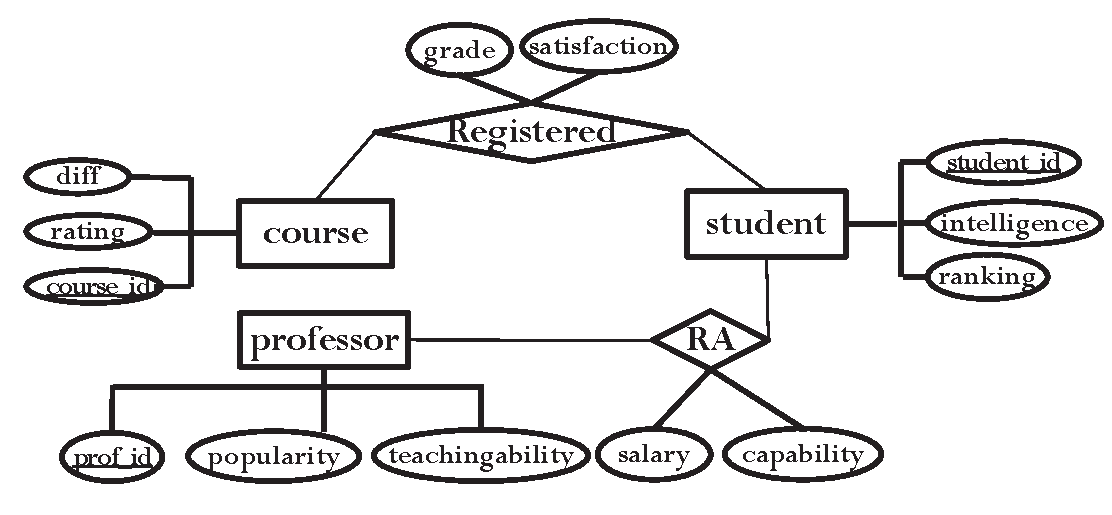
\includegraphics{university-schema.pdf} 
 } 
\caption{A relational ER Design for a university domain.}
 \label{fig:university-schema}
\end{figure}
\begin{figure}[htbp] %  figure placement: here, top, bottom, or page
 \centering
\resizebox{0.4\textwidth}{!}{
 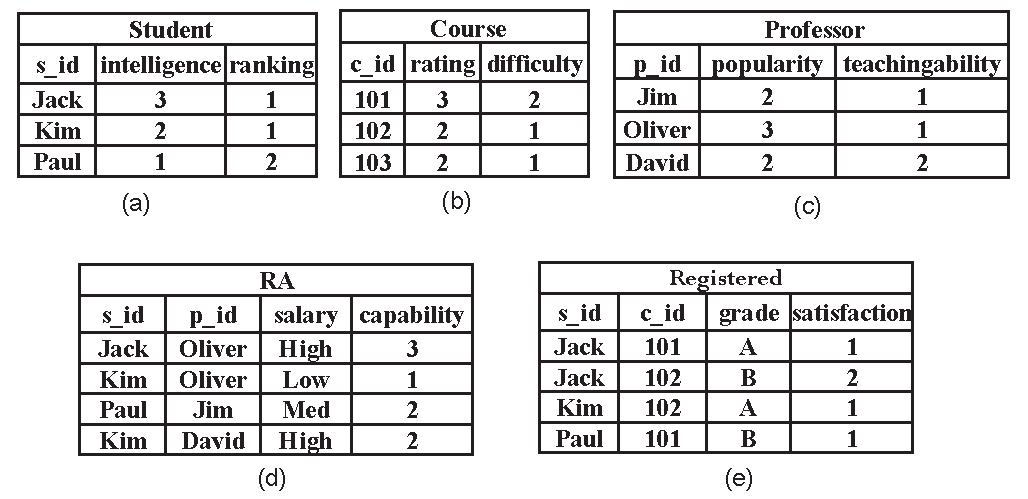
\includegraphics[width=0.5\textwidth]{university-tables.pdf} 
} 
\caption{Database Table Instances: (a) $\student$, (b) $\course$, (c) $\prof$, (d) $\ra$, (e) $\reg$.  
}
 \label{fig:instance}
\end{figure}


\subsection{Translating Entity-Relationship Models Into Functors}
 We assume a standard \textbf{relational schema} containing a set of tables, each with key fields, %typically
descriptive attributes, and possibly foreign key pointers. 
A \textbf{database instance} specifies the tuples contained in the tables of a given database schema. 
We assume that tables in the relational schema can be divided into {\em entity tables} and {\em relationship tables} (ER model) \cite[Ch.2.2]{Ullman1982}.
%This is the case whenever a relational schema is derived from an entity-relationship model  
 Figure~\ref{fig:university-schema} and Figure~\ref{fig:instance} show an ER diagram and an instance for a toy university domain, respectively. 
%An ER diagram shows entity sets as boxes, relationships between entities as diamonds, and attributes as ovals.
% Figure~\ref{fig:instance} shows a database instance for this ER diagram. 
%An ER diagram for single-table data would contain just one entity set box with attributes, and no relationships. 
Our approach is to translate the components of the ER diagram into random variables for statistical analysis \cite{Heckerman+al:SRL07}. The translation of an ER diagram into a set of functors converts each element of the diagram into a functor, except for entity sets and key fields. Table~\ref{table:translation} illustrates this translation.


%The functor formalism is rich enough to represent the constraints of an entity-relationship schema via the following translation: Entity sets correspond to populations, descriptive attributes to attribute functors, relationship tables to relationship functors, and foreign key constraints to type constraints on the arguments of relationship predicates. %, distinguishing attributes of entities ($\eatts$) and attributes of relationships ($\ratts$). 


%\begin{table}[btp] \centering
%\resizebox{0.4\textwidth}{!}{
%\begin{tabular}[c]
%{|l|c|l|l|}\hline
% ER Design &Type & Functor &\RRV \\\hline
%    \begin{tabular}{l}Entity \\Tables\end{tabular}&\begin{tabular}{l}Population \\Variables \end{tabular} & Student, Course & S, C \\\hline
%    \begin{tabular}{l}Relation \\Tables \end{tabular}&RNodes &RA & RA(P,S) \\\hline
%   \begin{tabular}{l}Entity \\Attributes \end{tabular}&1Nodes & intelligence, ranking &\begin{tabular}{l} \{intelligence(S), ranking(S)\}  \\=1Nodes(S) \end{tabular} \\\hline
%  \begin{tabular}{l} Relationship \\Attributes \end{tabular}&2Nodes & teachingability, salary &\begin{tabular}{l}   \{teachingability(P,S), salary(P,S)\}  \\= 2Nodes(RA(P,S))\end{tabular}\\\hline
%   
%\end{tabular}
%}
% % end scalebox
%\caption{Translation from ER Diagram to Relational Random Variable. \textbf{OS fix table}
% \label{table:translation}}
%\end{table}
\begin{table}[btp] \centering
\resizebox{0.4\textwidth}{!}{
\begin{tabular}[c]
{|l|c|l|l|}\hline
 ER Design &Type & Functor &\RRV \\\hline
    \begin{tabular}{l}Entity \\Tables\end{tabular}&\begin{tabular}{l}Population \\Variables \end{tabular} & Student, Course & $\S, \C$ \\\hline
    \begin{tabular}{l}Relation \\Tables \end{tabular}&Relationship &RA & RA($\P$,$\S$) \\\hline
   \begin{tabular}{l}Entity \\Attributes \end{tabular}&1Attributes & intelligence, ranking &\begin{tabular}{l} \{intelligence($\S$), ranking($\S$)\}  \\=1Attributes($\S$) \end{tabular} \\\hline
  \begin{tabular}{l} Relationship \\Attributes \end{tabular}&2Attributes & capability, salary &\begin{tabular}{l}   \{capability($\P, \S$), salary($\P, \S$)\}  \\= 2Attributes(RA($\P, \S$))\end{tabular}\\\hline
   
\end{tabular}
}
 % end scalebox
\caption{Translation from ER Diagram to Relational Random Variable. %\textbf{OS fix table}
 \label{table:translation}}
\end{table}

\begin{figure}[htbp] %  figure placement: here, top, bottom, or page
 \centering
\resizebox{0.4\textwidth}{!}{
 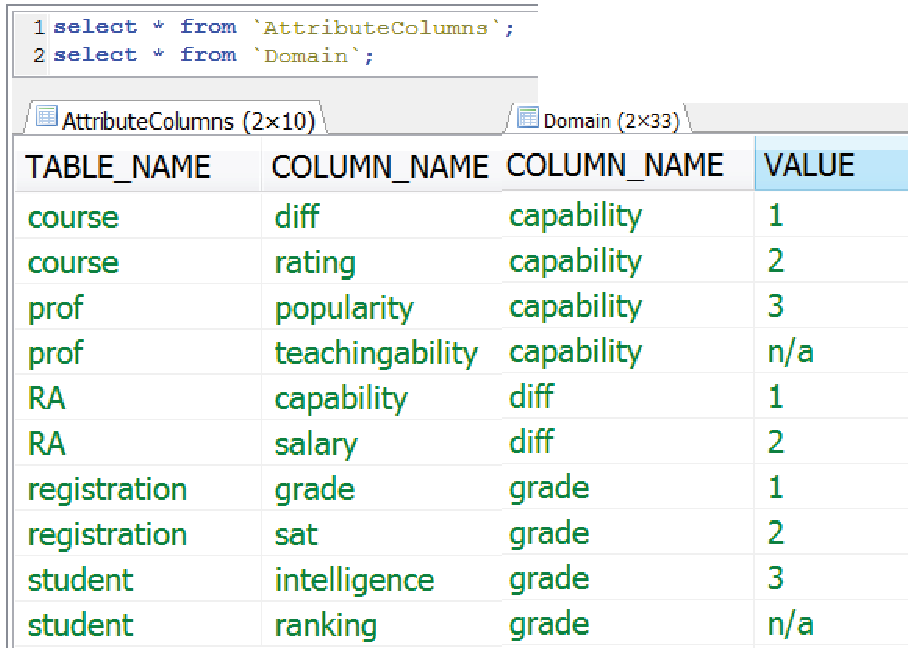
\includegraphics[width=0.5\textwidth]{attribute-domain.pdf} 
} 
\caption{The metainformation about attributes represented in database tables.  Left: The table $\it{AttributeColumns}$ specifies which tables and columns that contain the functor values observed in the data. The column name is also the functor ID. Right: The table $\it{Domain}$ lists the domain for each functor.
}
 \label{fig:attributes}
\end{figure}

There are different types of functors corresponding to the different types of ER diagram components. The simplest type represents an attribute of an entity set. We refer to such functors as \textbf{1Attributes}. In Figure~\ref{fig:university-schema}, there are six 1Attributes corresponding to attributes of Professors (2), Students (2), and Courses (2). 
%The primary keys (p\_id, s\_id, c\_id) are identifiers that are not treated as random variables. 
The metainformation about 1Attributes can be stored in a database table as shown in Figure~\ref{fig:attributes}. 
1Attributes correspond to {\em columns}. These are the only functors that appear in single-table data. 
%, just as random variables in single-table data do. 

Relationship functors have the Boolean domain $\{\true,\false\}$. Relationship functors correspond to {\em tables}, not columns. There are two relationship variables in the diagram~\ref{fig:university-schema} corresponding to the $\it{Registered}$ and $\it{RA}$ relationships. A relationship table stores the information about which entities are related to each other in a certain way. For example, the database instance of Figure~\ref{fig:instance} represents that student Jack took course 101, and that student Kim did not take course 101.
 Including a relationship random variable in a statistical model allows the model to represent uncertainty about whether or not a relationship exists \cite{linkGetoor2003}. 
%This supports applications like link prediction, (e.g., predicting whether two users are friends, \cite{Liben-Nowell2007}), and multiple link analysis for finding correlations among relationships (e.g., if user $u$ performs a web search for item $i$, is it likely that $u$ watches a video about $i$ ?). 
%
%Managing relationships raises several new issues compared to managing single-table column-based variables. 
To relate a relationship variable to the original relationship data, we need to store pointers to the related entity sets as metainformation. 

We refer to attributes of relationships as \textbf{2Attributes}. In Figure~\ref{fig:university-schema}, there are four 2Attributes corresponding to attributes of Registered (2) and RA (2). An important issue for relational data is that the values of descriptive attributes of relationships are undefined for entities that are not related. Following \cite{Russell2010}, we represent this by introducing a new constant $\it{n/a}$ in the domain of a 2Attribute; see Figure~\ref{fig:attributes} (right). RRV's are called \textbf{1Variables} if their functor is a 1Attribute, \textbf{2Variables} if it is a 2Attribute, and \textbf{RVariables} if it is a relationship.
%\cite{BLOG}, 
%$\it{capability(\P,\S)} = n/a $
%we indicate this by writing 
%%$\it{grade}(\s,\c) = n/a$ 
%$\it{capability(\P,\S)} = n/a $ for a reserved constant $\it{n/a}$. 
%The assertion $\it{capability(\P,\S)}$ = n/a is therefore equivalent to the assertion that $\ra(\P,\S) = \false$.

%\subsection{Generating Default Relational Random Variables}

%We use upper case for Boolean-valued variables with domain $\{\true,\false\}$, such as RVariables. We use
%lower case for other random variables. 

%\subsection{Population Variables and SQL Implementation} \label{sec:pvariables}
%
%The Schema Analyzer combines population variables with functors to obtain full RRVs. The random variable database specifies a set of population variables. A population variable refers to an entity set. With each population variable, we store a pointer to the original entity set as metainformation. For example, the $\it{S}$ population variable is associated with the the $\it{Student}$ table in the original database. 
%%In the example of Figure~\ref{fig:university-schema}, the type/foreign key constraints on the functors determine which population variables to add, as shown in Table~\ref{table:translation}. In this case adding population variables to functors enhances readability but is redundant given the type information in the schema.
%
%If the database schema contains a self-relationship, 
%by default, the Schema Analyzer creates three RVariables and three population variables for the self-relationship. A self-relationship relates two entities of the same type.
%Neville and Jensen provide evidence that self-relationships are very common, so it is important to accommodate them in a statistical model \cite{Neville2007}.
%%
%%Some relational schemas require more than one population variable for the same entity set. 
%%This additional expressive power becomes important in the presence of {\em self-relationships} \cite{Heckerman+al:SRL07}. 
%%A self-relationship relates two entities of the same type.
%%%, when we need to introduce more than one relationship node for the relationship functor. 
%%For example, the Mondial database contains a self-relationship $\it{Borders}$ that relates two countries, as shown in the ER diagram Figure~\ref{fig:mondial-er}. As they lead to major conceptual differences between relational and single-table data, we discuss self-relationships in some detail. Neville and Jensen provide evidence that self-relationships are very common, so it is important to accommodate them in a statistical model \cite{Neville2007}. Self-relationships give rise to {\em relational autocorrelations,} where the attribute value of an entity depends probabilistically on the attribute value of related entities \cite{Neville2007}. 
%%Relational autocorrelations are analogous to temporal autocorrelations in time series analysis, where there is a correlation between the value of a quantity at one time and the value of the same quantity at another. An autocorrelation cannot be represented in a model that contains only one random variable referring to the quantity in question. For time series, a common solution is to introduce {\em two} distinct random variables  that refer to the same quantity, but at different times. For instance, we may have two random variables $\it{temperature}_{t}$ and $\it{temperature}_{t+1}$. Similarly, to represent a relational autocorrelation between the continents of two different countries, we may introduce two random variables $\it{continent}_{\C_{1}}$ and $\it{continent}_{\C_{2}}$. The index notation can equivalently be replaced by function notation, writing $\it{continent}(\C_{1})$ and $\it{continent}(\C_{2})$ \cite{Milch2005}. 
%%%This leads to the concept of a relational random variable as previously defined. 
%%%
%%%In the ER diagram, there are two lines from the $\it{Countries}$ entity set to the $\it{Borders}$ relationship set 
%%%The ring structure may be represented with two different population variables that each refer to the $\it{Countries}$ entity set. 
%%The corresponding relationship random variable is $\it{Borders}(\C_{1},\C_{2})$. The different positions of the 1st-order variables can represent different roles in the relationship. A random variable for a descriptive 2Attribute can also be represented using population variables, for instance $\it{Border\_Length}(\C_{1},\C_{2})$. %\textbf{OS: add ER diagram for this simple Mondial example}. 
%%This notation is expressive enough to represent autocorrelations. 
%%For instance, the association rule
%%
%%\begin{small}
%%$\it{continent}(\C_{1}) = \it{Europe}, \it{Borders}(\C_{1}, \C_{2}) = \true \rightarrow \\\it{continent}(\C_{2}) = \it{Europe}$
%%\end{small}
%%
%%expresses that if two countries are neighbors and one is in Europe, the other country is likely to be in Europe. 
%%
%%Some complex patterns require more than one relationship variable for the same relationship functor. For instance, representing transitivity requires three relationship variables.
%%%as in 
%%%$$\it{Borders}(\C_{1}, \C_{2}) = \true,  \it{Borders}(\C_{1}, \C_{3}) = \true \rightarrow \it{Borders}(\C_{1}, \C_{3}) = \true.$$
%%%Since we introduce two population variables referring to the same entity set, we need to duplicate the 1Nodes for that entity set. 
%%%This allows the logical language to represent that attributes of neighboring countries influence each other, 
%%%%Using a second relationship node with the $\it{Borders}$ functor allows us to represent such influences, 
%%%for instance in the following rule
%%%$$\it{continent}(\C_{1}) = \it{Europe}, \it{Borders}(\C_{1}, \C_{2}) = \true \rightarrow \it{continent}(\C_{2}).$$
%%If the database schema contains a self-relationship, 
%%by default, the Schema Analyzer creates three RVariables and three population variables for the self-relationship.
%%%, together with the applicable 1Variables.
%%% (e.g., $\it{continent}(\C_{3}$).
%%It adds one population variable for each role in the relationship. For each population variable there is a separate set of corresponding 1Variables. In the Mondial example, there are two 1Variables $\it{continent}(\C_{1})$ and $\it{continent}(\C_{2})$.
%%\begin{figure}[htbp] %  figure placement: here, top, bottom, or page
%% \centering
%%\resizebox{0.4\textwidth}{!}{
%% 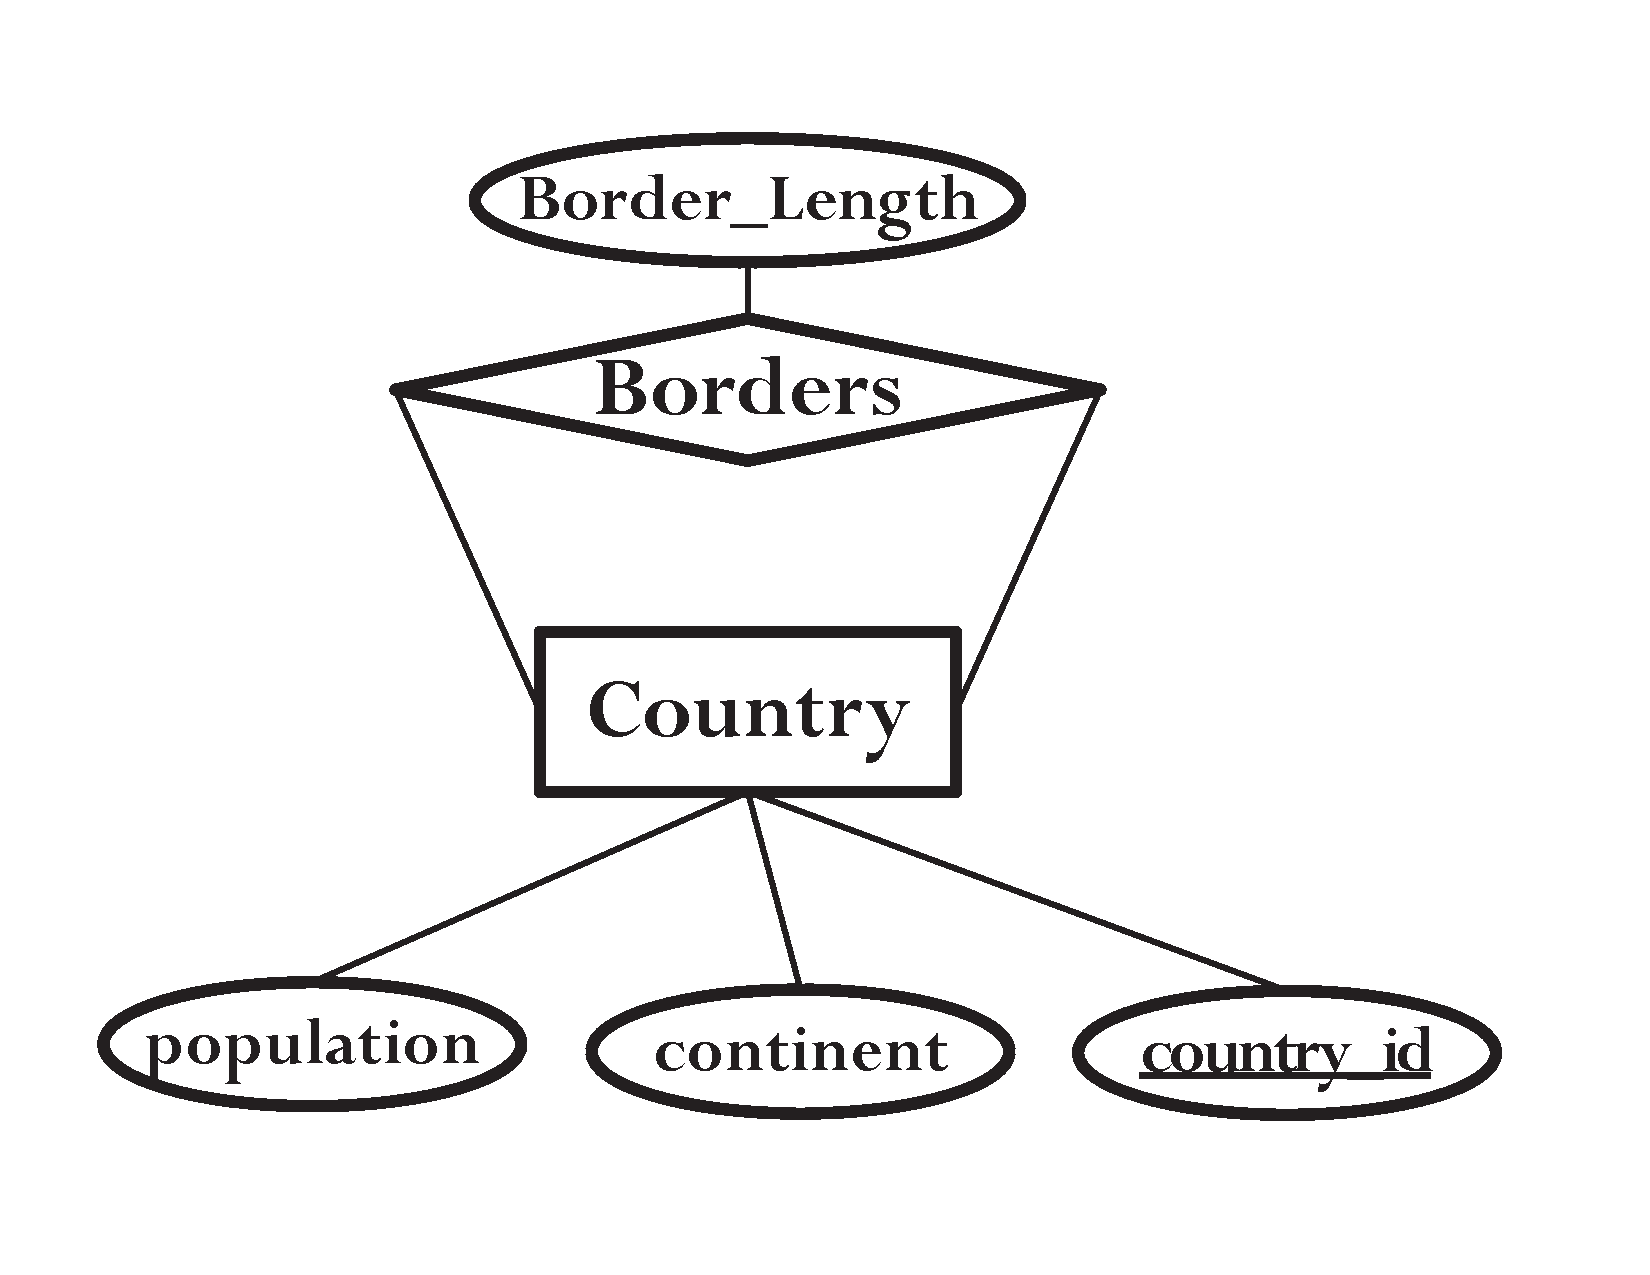
\includegraphics[width=0.4\textwidth]{mondial-er.pdf} 
%%} 
%%\caption{The ER diagram for Mondial database. $\it{Borders}$ is a self-relationship. 
%%}
%% \label{fig:mondial-er}
%%\end{figure}
%
%%\subsection{SQL Implementation}
%The metainformation about the random variables is stored in the \textbf{random variable database} ($\RVD$). The relational schema of the $\RVD$ is shown in Figure~\ref{fig:rv_db}. %\textbf{OS: make 6 relations}. 
%The relational schema of the original database is represented in tables in the database system catalog. Given that both the system catalog and the $\RVD$ are databases, we can use SQL to transfer information from one to the other. %\textbf{OS make SQL query} 
%We show some of the SQL queries in the Schema Analzyer that the metainformation about 1Attributes from the system catalog in our  university example. The full SQL script, 
%%included in the appendix, 
%also constructs tables for 2Attributes and relationship variables, and recognizes self-relationships by using foreign key pointer information. Figure~\ref{fig:rv_db} shows tables that are constructed by the SQL queries in the Schema Analyzer.
%%The full script is included in the supplementary material. 
%
%The first SQL query shows the construction of population variables in our university example. 
%%It assume the existence of a KeyColumns table that contains triples (TableName, ColumnName, ConstraintName) to record which column in which table is associated with a key constraint. 
%%The query uses this information to identify tables with just one primary key column, which represent entity sets. 
%%The name of such tables is concatenated with an index to produce indexed population variables as discussed in Section~\ref{sec:pvariables}. 
%The second query constructs a table listing 1Variables, which are relational random variables representing 1Attributes, identified by a 1Attribute name and a population variable. 
%The use of the natural join operation to combine functors with population variables illustrates how relational algebra elegantly supports defining new statistical objects from existing statistical objects.
%%After the random variable database has been created from the system catalog, the user  can add or substract relational random variables depending on the statistical patterns of interest.  such as WinBugs or mode declarations in Aleph.
%%As we discuss next, the remaining components of MRLBase depend only on the metainformation in the $\RVD$ database, not on the system catalog.
%\begin{alltt}
%CREATE TABLE PVariables AS  SELECT 
%CONCAT(EntityTables.TABLE_NAME, `0') AS pvid,
%EntityTables.TABLE_NAME FROM
%(SELECT distinct TABLE_NAME, COLUMN_NAME 
%FROM   KeyColumns T WHERE
%1 = (SELECT  COUNT(COLUMN_NAME)   
%FROM   KeyColumns T2  WHERE     
%T.TABLE_NAME = T2.TABLE_NAME
%AND CONSTRAINT_NAME = 'PRIMARY')) 
%as EntityTables 
%
%CREATE TABLE 1Variables AS
%SELECT CONCAT(`\`', COLUMN_NAME,
% `(', pvid, `)', `\`') AS 1VarID,
%COLUMN_NAME,   pvid  FROM    
%PVariables   NATURAL JOIN  AttributeColumns;
%\end{alltt}
%
%\begin{figure}[htbp]
%\begin{center}
%\resizebox{0.5\textwidth}{!}{
%%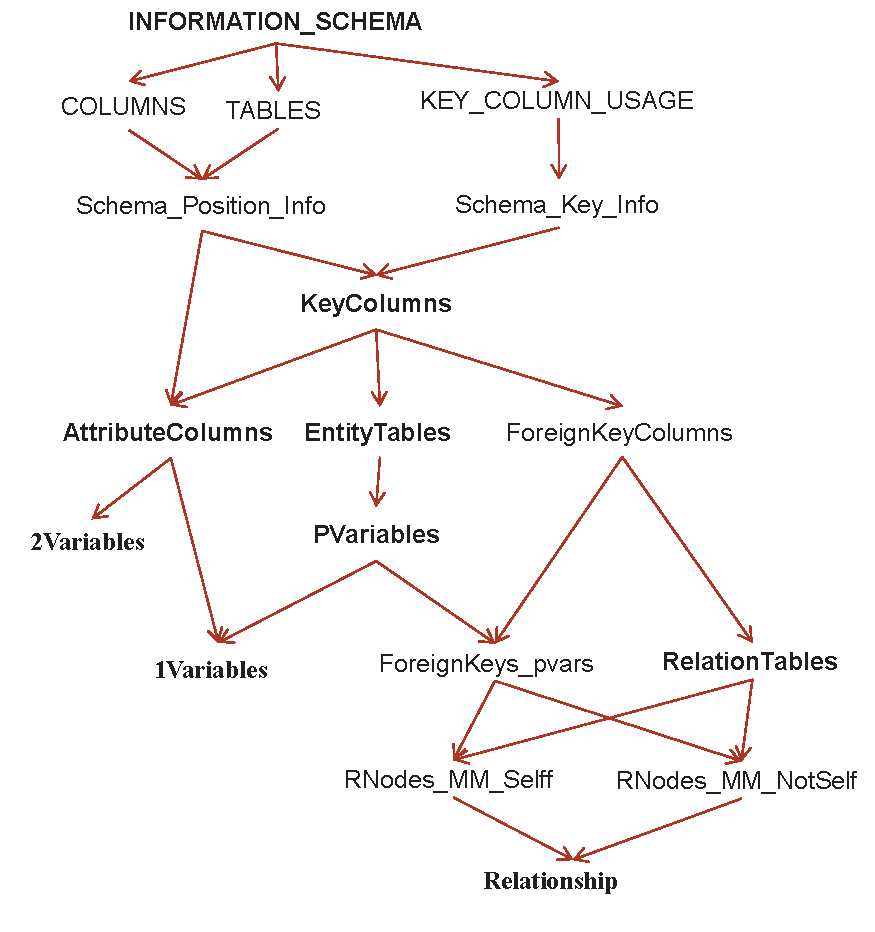
\includegraphics[width=0.5\textwidth]{rv_db.pdf} %move to the appendix
%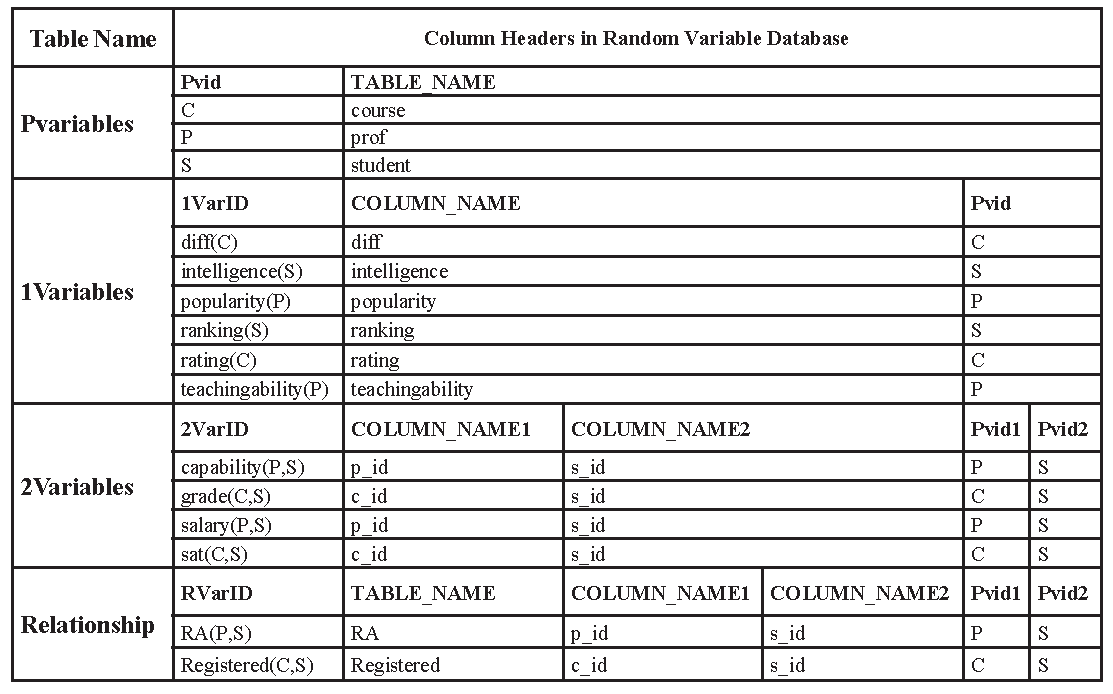
\includegraphics[width=0.5\textwidth]{rv_db_tables.pdf}
%}
%\caption{Metainformation: Main Tables in the Random Variable Database $\RVD$. 2Variables are relational random variables that represent attributes of binary relationships.
%\label{fig:rv_db}}
%\end{center}
%\end{figure}
%
%\section{The Count Manager} 
%A key service for machine learning that a data management system needs to provide is counting how many times a given pattern is instantiated in the data. Such counts are known as {\em sufficient statistics} \cite{Graefe1998}. 
%%Many statistical machine learning algorithms do not require full access to the original data, but only to sufficient statistics (hence the name ``sufficient''). So if a database management system is extended to provide sufficient statistics on demand, a learning algorithm for single-table data can be applied to relational database with few modifications. 
%%
%A novel aspect of MRLBase is managing sufficient statistics in the RDBMS, which has several important advantages. 
%%There are several reasons for employing an RDBMS for gathering sufficient statistics. 
%%(1). The machine learning application saves expensive data transfer by executing count operations in the database server space rather than local main memory. (2) SQL optimizations for aggregate functions such as SUM and COUNT can be leveraged. (3) Sufficient statistics can be computed once and stored/cached for future reuse in the RDBMS. For many datasets, the number of sufficient statistics runs in the millions and is too big for main memory \cite{Moore1998}.  
%%
%%An RDBMS provides disk storage and fast access for large numbers of sufficient statistics. 
%Previous work has exploited these advantages for single-table data \cite{Ordonez2010}. 
%We discuss how to compute sufficient statistics for a more general situation where sufficient statistics combine information {\em across} different tables in the relational database. In SQL terms, this requires combining aggregate functions with table joins. 
%
%
%\subsection{Relational Contingency Tables}
%%Our starting point is the observation that a statistical learning algorithm like a Bayes net learner does not require an enumeration of individuals tuples, but only {\em sufficient statistics} \cite{Heckerman1995,Schulte2011}. 
%%It is well-known in machine learning that a statistical learning algorithm like a Bayes net learner does not require an enumeration of individuals tuples, but only {\em sufficient statistics} \cite{Heckerman1995,Schulte2011}. 
%
% %A contingency table is defined as follows.
%%The Bayes net is learned from the contingency table. 
%
%%The count column in the $\ct$-table represents the number of instantiations for a given tuples of values in a row in the input database. 
%Sufficient statistics can be represented in {\em contingency tables} as follows \cite{Moore1998}. 
%Consider a fixed list of relational variables.
%%$\R_{1}, R_{2},\ldots,R_{m}$, and attribute nodes $\functor_{1},\ldots,\functor_{j}$. 
%A \textbf{query} is a set of $(variable = value)$ pairs where each value is of a valid type for the variable. 
%The \textbf{result set} of a query in a database $\D$ is the set of instantiations of the population variables such that the query evaluates as true in $\D$.
%For example, in the database of Figure~\ref{fig:instance} the result set for the query 
%%$(\it{intelligence}(\S) = 2$, $\it{rank}(\S) = 1$, $\it{rating}(\C) = 3$, $\it{diff}(\C) = 1$, $\reg(\S,\C) = F)$
%$(\it{intelligence}(\S) = 2$, $\it{rank}(\S) = 1$, $\it{popularity}(\P) = 3$, $\it{teachingability}(\P) = 1$, $\ra(\P,\S) = T)$ 
%is the singleton $\{\langle \it{kim}, \it{Oliver}\rangle\}$. 
%% $\{\langle \it{kim}, \it{101}\rangle\}$
%The \textbf{count} of a query is the cardinality of its result set. 
%
%Every set of variables $\set{V} \equiv \{\V_{1},\ldots,\V_{n} \}$ has an associated \textbf{contingency table} ($\cttable$) denotes by $\cttable(\set{V})$. %$CT(\set{V})$. 
%This is a table with a row for each of the possible assignments of values to the variables in $\set{V}$, and a special integer column called $\qcount$. 
%The value of the $\qcount$ column in a row 
%corresponding to $V_{1} = v_{1},\ldots,V_{n} = v_{n}$ records the count of the 
%corresponding query. 
%Figure~\ref{fig:ct} shows the contingency table for the university database. The \textbf{contingency table problem} is to compute a contingency table for a target set of variables $\set{V} $ and a given database $\D$. 
%%Machine learning algorithms can leverage this capability in several different ways. A pre-counting approach computes a joint contingency table for all relational random variables at once \cite{Moore1998,Qian2014a}. Another possibility is to use postcounting \cite{lv2012}: Rather than precompute a large contingency table prior to learning, compute many small contingency tables for  small subsets of variables on demand during learning. I
%%n this paper, we describe an approach to compute contingency tables that leverages SQL capabilities. First, 
%MRLBase stores contingency tables as first-class database tables.
% %as in \cite{Qian2014a}. 
% The column headers of a contingency table are IDs for the relational random variables, plus an integer-valued count column. 
%
%%The value of a relationship attribute is undefined for entities that are not related.
%%Following \cite{Milch2005}, %\cite{BLOG}, 
%%%$\it{capability(\P,\S)} = n/a $
%%we indicate this by writing 
%%%$\it{grade}(\s,\c) = n/a$ 
%%$\it{capability(\P,\S)} = n/a $ for a reserved constant $\it{n/a}$. 
%%The assertion $\it{capability(\P,\S)}$ = n/a is therefore equivalent to the assertion that $\ra(\P,\S) = \false$.
%%For example, if student $\s$ is not registered in course $\c$, the value of $\it{grade}(\s,\c)$ is undefined. 
%
%
%\begin{figure}[htbp]
%\begin{center}
%\resizebox{0.5\textwidth}{!}{
%%%!%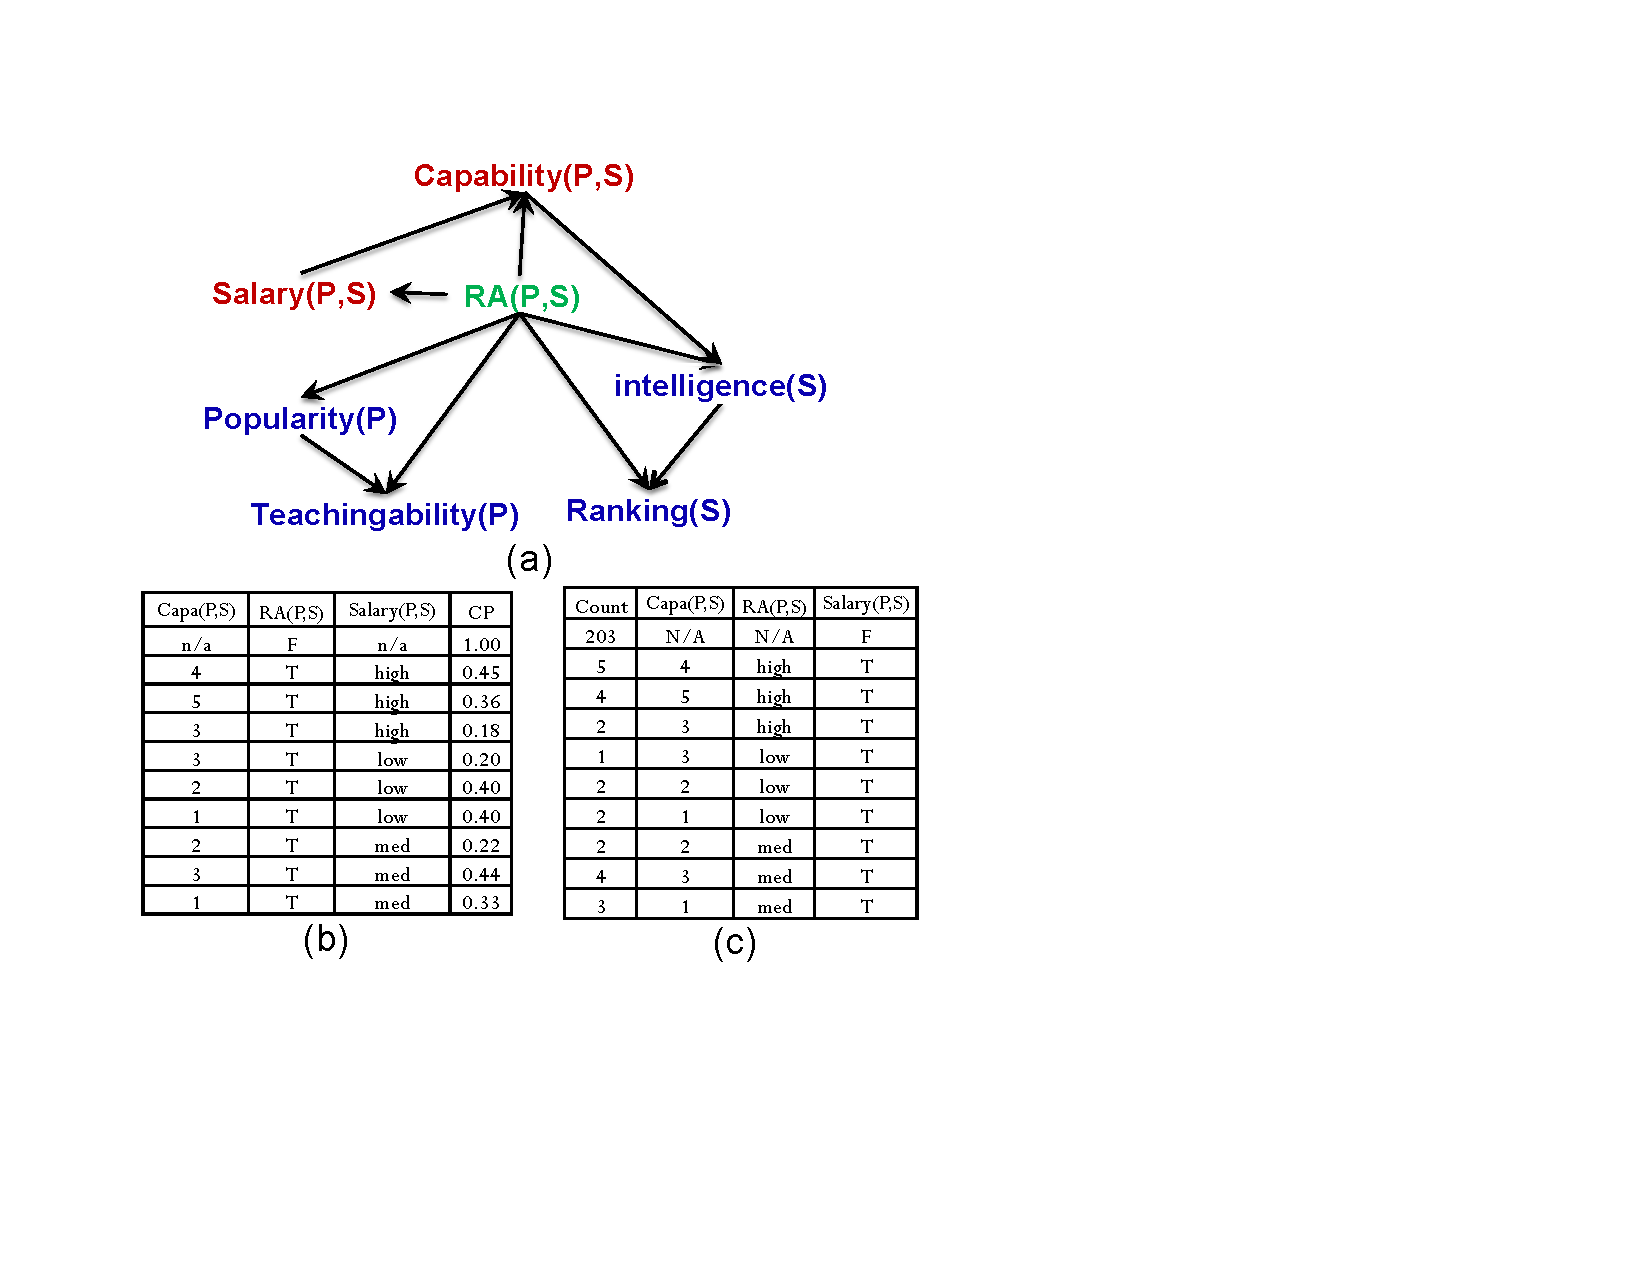
\includegraphics[width=1\textwidth]{pbn}
%%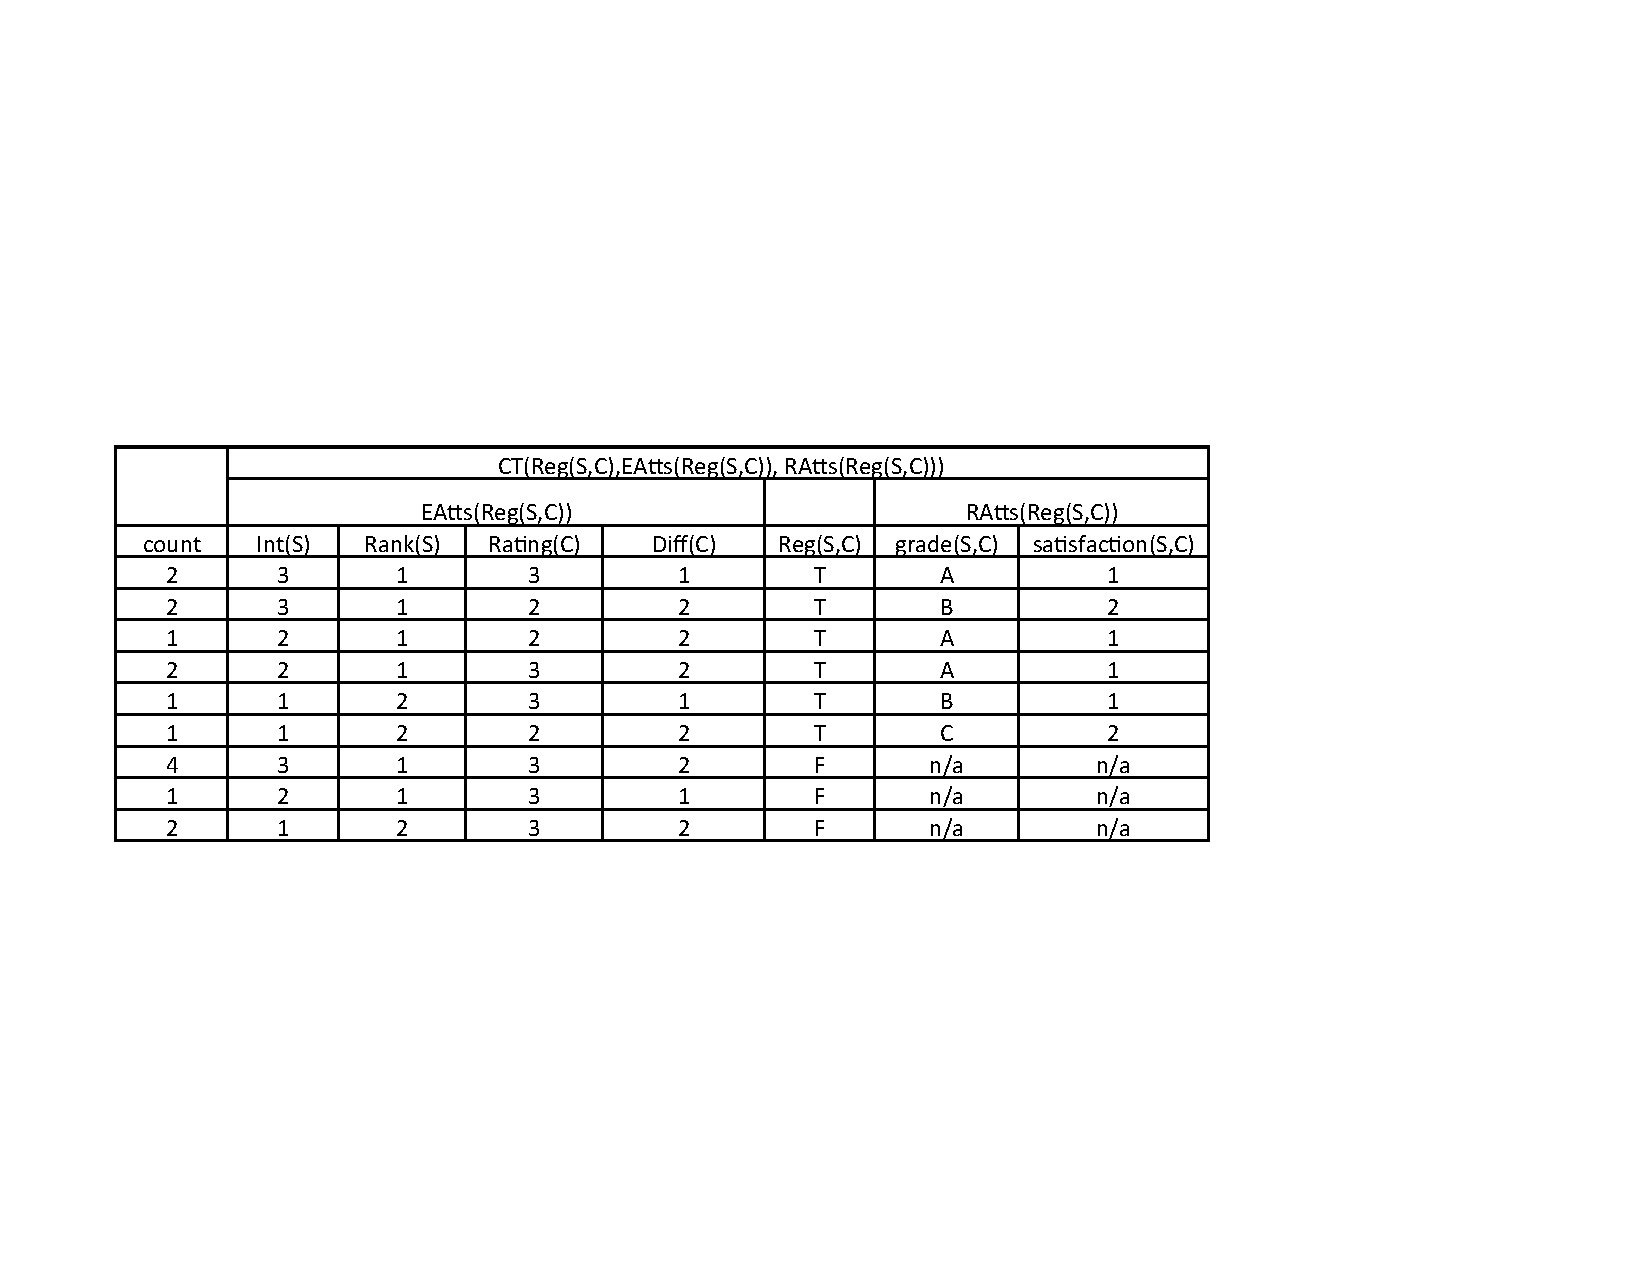
\includegraphics{figures/ct-table.pdf}
%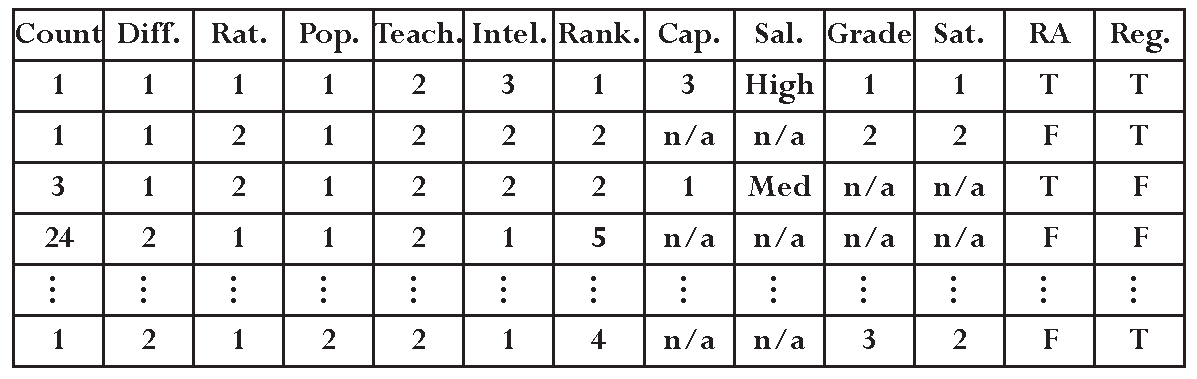
\includegraphics[width=0.5\textwidth]{uni-ct-table.pdf}
%}
%\caption{The contingency table for the university database. % for the attribute-relation table of Figure~\ref{fig:university-tables}
%Each row defines a query and its instantiation count in the database. For legibility, we show only functors, not the population variables. %one possible assignment of such variables with its count. 
%% where for illustration we have added counts for another student like Jack and another course like 103.
%%use partial real table
%\label{fig:ct}}
%\end{center}
%\end{figure}
%
%%A \textbf{conditional contingency table}, written 
%%$$\ct(V_{1},\ldots,V_{k}|V_{k+1} = v_{k+1},\ldots, V_{k+m} = v_{k+m})$$
%%is the contingency table whose column headers are $V_{1},\ldots,V_{k}$ and whose counts are  defined by subset of instantiations that match the conditions to the right of the $\vert$ symbol.  %  \textbar 
%
%
%
%%To illustrate the SQL-based approach, we examine the following problem: precomputing a contingency table for all relational random variables that are associated with a given chain of relationships. A relationship chain is a list $$[\Relation_{1}(\argterms_{1}),\ldots,\Relation_{k}(\argterms_{k})]$$
%% of relationship variables such that each relationship variable shares at least one first-order variable with the preceding terms. In SQL terms, a relationship is formed by following foreign key pointers from one relationship table to the next. Sufficient statistics for relationship chains are important for discovering correlations between the attributes of entities that are related by paths of a certain type \cite{Getoor2007c} (called ``metapaths'' in \cite{Sun2012}). 
% 
%\subsection{Contingency Tables in SQL} The \textbf{Count Database} (CDB) stores a set of contingency tables each defined as a view. We describe how to create these views using SQL.  
%Each row in a $\cttable$ represents the count for a conjunctive query in a logical calculus; we refer to these as count-conjunction queries which 
%%It is well-known that conjunctive queries in a logical calculus 
%can be algorithmically translated into relational algebra queries and hence into an SQL query \cite{Ullman1982}.
%Our approach uses SQL itself to construct the count-conjunction query. We refer to this construction as an SQL \textbf{metaquery}. Metaqueries share the advantages of SQL over using a general programming language 
%%discussed in Section~\ref{sec:design}
%: They are compact, portable, and support automatic updates through the view mechanism.
%% (1) Succinctness and portability: Given the metainformation in the random variable database, the meta query is short, mainly requires a few natural joins. The meta query requires only standard SQL, whereas a translation in an application language (e.g., Java) would have to be ported for each different application language. (2) Automatic Update: We can store the result of the meta query as a database view. 
%% This means that changes in the original database schema are propagated to contingency tables. For instance, if a column $\it{gpa}$ is added to the $\it{Student}$ table in the original database schema, then the view definition adds this column automatically to contingency tables derived from the $\it{Student}$ table.

\section{Count Queries and Machine Learning Tasks}

In terms of computational efficiency, the key issue for BN learning is computing event counts or sufficient statistics. Such counts are necessary for several machine learning tasks, such as:

\begin{itemize}
\item parameter estimation
\item computing the BN likelihood function
\item classification
\item computing the pseudo-likelihood score of a candidate BN.
\end{itemize}
  
[elaborate]

Multi-relational data raise special challenges in computing sufficient statistics [copy from CIKM]. Our goal in this section is to show how SQL capabilities can be leveraged to address these challenges. 


Sufficient statistics can be computed using an \textbf{SQL count query}, which has the form 
\begin{alltt}
%CREATE CT-table(<VARIABLE-LIST>) AS
SELECT COUNT(*) AS count, <VARIABLE-LIST>
FROM TABLE-LIST
GROUP BY VARIABLE-LIST
WHERE <Join-Conditions>, <restrictions>
\end{alltt}

\subsection{Bayesian network multi-relational parameter estimation}

\subsection{Bayesian network multi-relational likelihood computation}

\subsection{Multi-relational Classification with Bayesian networks}

\subsection{Bayesian network multi-relational pseudo-likelihood computation}

\section{Metaqueries: generating dynamic count queries}

The \textbf{count query generation problem} is to generate a correct SQL count query for a given set of variables and restrictions that come from the machine learning client. [This needs to be done dynamically.] The query generation program should use metainformation about the random variables to automatically find the correct tables to join and the appropriate join conditions. Our solution is to stay within SQL and use an SQL \textbf{meta query} to generate the required SQL count query. 



%As the top level of  Figure~\ref{fig:flow} illustrates, 
%The required counts involving only true relationships can be computed using the standard SQL constructs COUNT(*) and GROUP BY. 
%The general form of these operations is the same for every input database. 
%The varying part is the list of columns to be included, which depends on the input database. 
%For a fixed database, the column lists can be hard-coded. 
%To achieve a general solution when the column list is not known in advance, we introduce a new approach that we refer to as an SQL \textbf{meta query}. 
%Thus an SQL meta query maps schema information to the components of another SQL query. 
 Given a list of $\RRV$'s as input, the meta query is constructed as follows from the metainformation in the random variable DB.  
\begin{description}
\item[FROM LIST] Find the tables referenced by the $\RRV$'s. An $\RRV$ references the entity tables associated with its population variables (see $\RVD.Pvariables$). Relational $\RRV$'s also reference the associated relationship table (see $\RVD.Relationship$). 
\item[WHERE LIST] Add join conditions on the matching primary keys of the referenced tables in the WHERE clause. The primary key columns are recorded in table $\RVD.KeyColumns$. 
\item[SELECT LIST] For each attribute $\RRV$, find the corresponding column name in the original database (see $\RVD.AttributeColumns$). Rename the column with the ID of the $\RRV$.
\end{description}

We represent a count-conjunction query of this form in 
four kinds of tables: the Select, From, Where and Group By tables. 
The Select table lists the entries in the Select clause of the target query, the From table lists the entries in the From clause, and similar for Where and GROUP BY tables. The entries of the Group By table are the same as in the Select table without the $\qcount$ column.
Given the four query tables, the corresponding SQL count query can be easily executed in an application or stored procedure to construct the contingency table.
% The metaquery accesses tables in the Relational Random Variable Database. %We omit further details due to space constraints.


Figure~\ref{fig:meta-query} shows an example of metaqueries for the university database. This metaquery defines a view that in turn defines a contingency table for the random variable list associated with the relationship table $\ra$. This list includes the 1Attributes of professors and of students, as well as the 2Attributes of the $\ra$ relationship. The resulting $\cttable$ is like that of Figure~\ref{fig:ct}, but without the $\it{Reg.}$ column and only with rows where the value of $\ra$ is true. This $\cttable$ can extended to include counts for when $\ra$ is false using the M\"obius Virtual Join~\cite{Schulte2014}.

\begin{figure}[htb]
\begin{center}
\resizebox{0.5\textwidth}{!}{
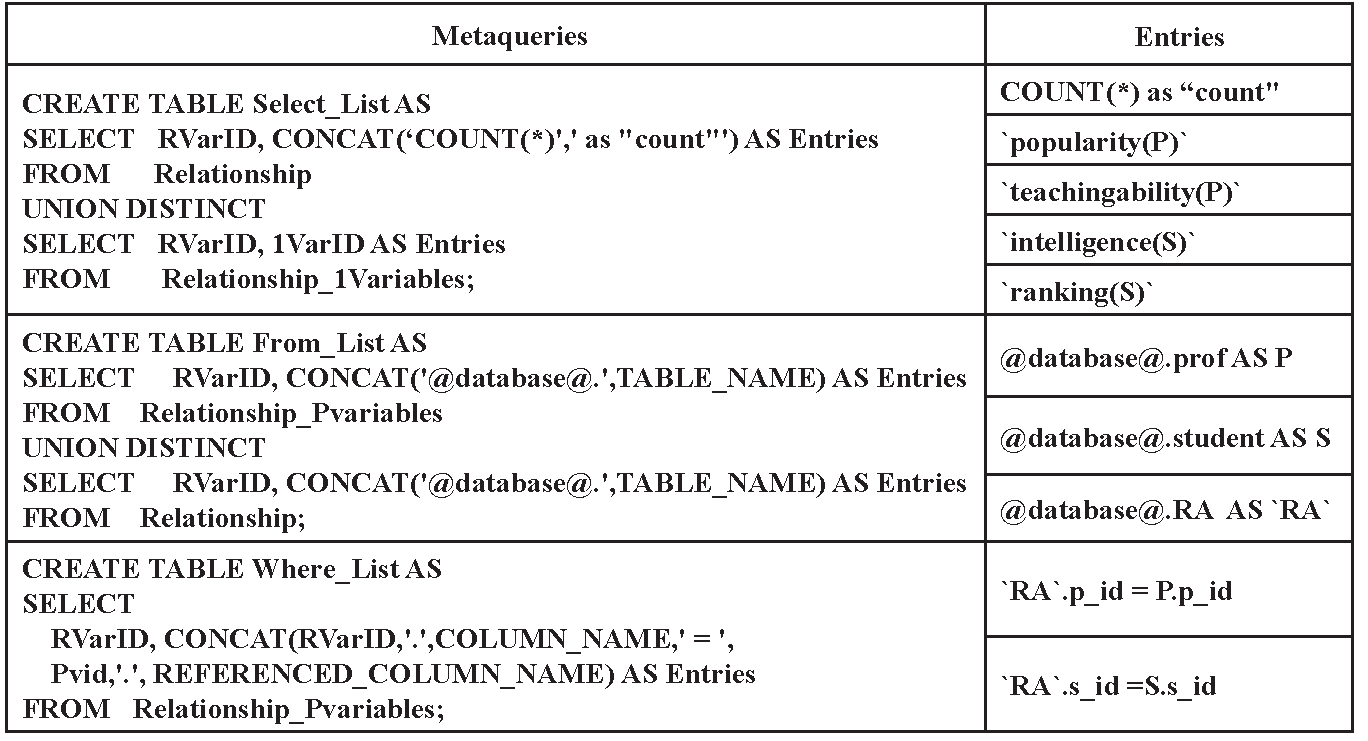
\includegraphics[width=0.5\textwidth]{meta-query.pdf}
}
\caption{Example of metaqueries and metaquery results based on university database. The parameter $\it{@database@}$ refers to the name of the input database. 
~\label{fig:meta-query} }
\end{center}
\end{figure}

\section{Bayesian network multi-relational structure learning}

\subsection{The Model Manager}

\subsection{Model Search}

\subsubsection{Model Selection Score}

\subsubsection{Model Optimization Search Algorithm}

\section{Evaluation}

\subsection{Parameter Estimation}

How many parameters, how long does it take.
Baseline: big join table?

\subsection{BN multi-relational likelihood computation}

How long it takes for a single pass.

\subsection{Classification}

How long it takes for single object. Total time in loop (testing scenario).

\subsection{Pseudo-likelihood}

Compare with classification loop.

\subsection{Model Learning}

How long, how accurate. Don't use pseudo-likelihood because that's the evaluation metric for accuracy. Baseline RDN-Boost. 

There is a large space of machine learning models, which require support for a diverse set of capabilities. We focus on the services that are required in almost all model selection tasks: 1) Estimating and storing parameter values. 2) Computing one or more model selection scores. %3) Inferring a model prediction for a set of test instances and scoring the model against the true values. 
%We also discuss model structure learning. 

Our case study describes how MRLBase can be used to implement a challenging machine learning application: Constructing a Bayesian network model for a relational database. 
Managing Bayesian networks are a good illustration of typical challenges and how RDBMS capabilities can address them because: (1) Bayesian networks are a structured graphical model. (2) BN parameters are localized and not simply a flat vector. (3) Bayesian networks are widely regarded as a very useful model class in machine learning and AI, that supports decision making and reasoning under uncertainty. At the same time, they are considered challenging to learn from data. (4) Database researchers have proposed Bayesian networks for combining databases with uncertainty \cite{Wang2008,Deshpande2007}. 
%
%After we have illustrated the our SQL-based approach for BN learning, we discuss how to apply it with other machine learning models.

\subsection{Bayesian Networks for Relational Data}
A {\bf Bayesian Network (BN)} is a directed acyclic graph (DAG) whose nodes comprise a set of random variables and conditional probability parameters.
The parameters of the BN  are the conditional probabilities of the form, $P(\it{child}|\it{parent\_values}$), that specify the probability of a child node value given an assignment of values to its parents. 
In this paper we consider only Bayesian networks whose nodes are relational random variables (called ``Parametrized Bayesian Networks'' in \cite{Poole2003}). When discussing a BN, we interchangeable refer to its nodes or to its random variables.
%If a Parametrized random variable appears in a Bayes net, we often refer to it simply as a node. 
Figure \ref{fig:pbn} shows a Bayesian network for the University domain (only considering the $\ra$ relationship for simplicity.) 
\begin{figure}[htbp] %  figure placement: here, top, bottom, or page
 \centering
\resizebox{0.4\textwidth}{!}{
 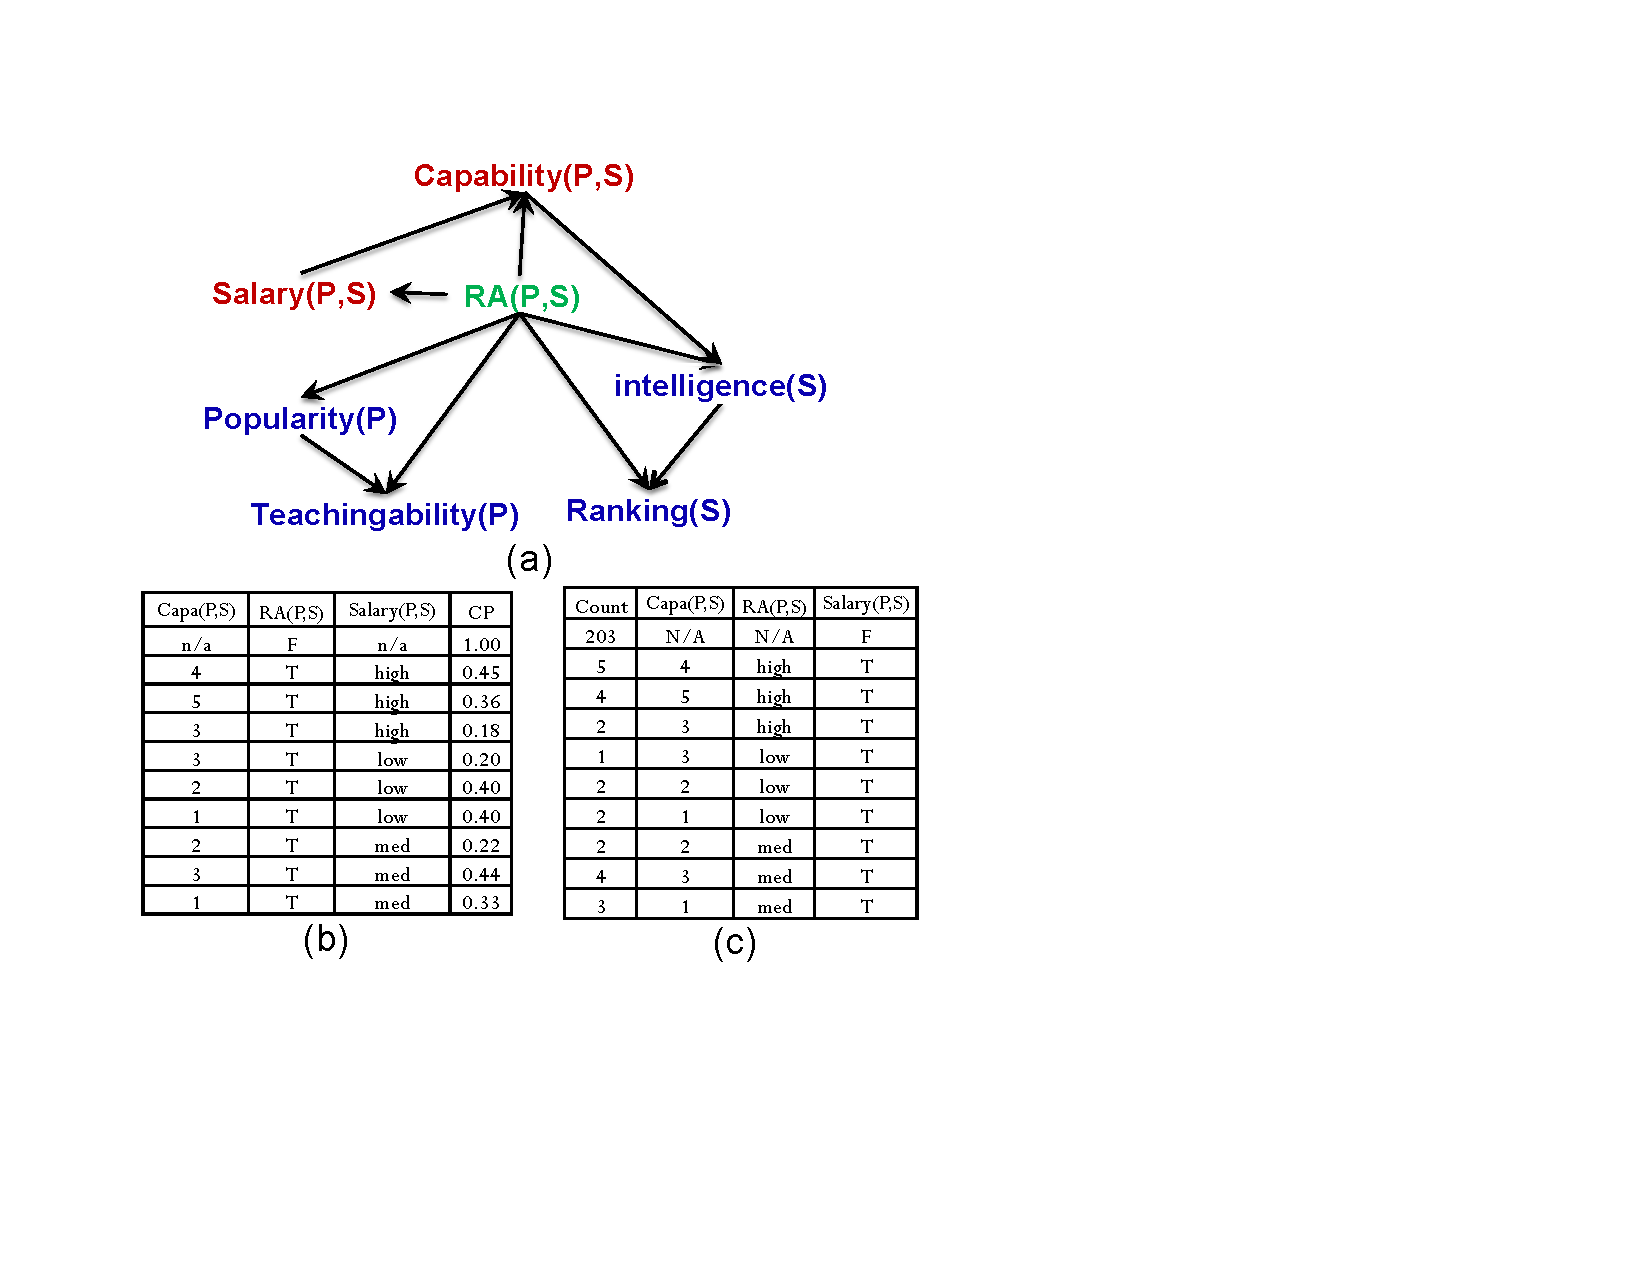
\includegraphics[width=0.5\textwidth]{pbn.pdf} 
} 
\caption{(a) Bayesian network for the University domain. (b) Conditional Probability table $Capability(\P,\S)\_\cptable$, for the node $Capability(\P,\S)$. Only value combinations that occur in the data are shown. (c) Contingency Table $Capability(\P,\S)\_\cttable$ for the node $Capability(\P,\S)$ and its parents. Both CP and CT tables are stored as database tables.
}
 \label{fig:pbn}
\label{fig:ct-cp-table}
\end{figure}


%\begin{figure}[htbp] %  figure placement: here, top, bottom, or page
% \centering
%\resizebox{0.4\textwidth}{!}{
% \includegraphics[width=0.5\textwidth]{ct-cp-table.pdf} 
%} 
%\caption{ct-cp-table}
% \label{fig:ct-cp-table}
%\end{figure}

%\subsection{Model Representation} 
\paragraph{SQL Representation} A Bayesian network structure is a directed graph that can be stored straightforwardly in a database table $\it{BayesNet}$ whose columns are $\it{child}$ and $\it{parent}$. The table entries are the IDs of relational random variables defined in the Relational Random Variable database. An entry such as $(\it{Capability}(\P,\S),\it{Salary}(\P,\S))$ means that $\it{Capability}(\P,\S)$ is a child of $\it{Salary}(\P,\S)$. This table is stored in the Models Database $\MDB$. The relational schema for the Models Database is shown in Table~\ref{table:mdb-schema}.
\begin{table}[tbp] \centering
 \begin{tabular}
[c]{|l|}\hline
$\it{BayesNet}$(\underline{$child$,$parent$})\\
$\it{@nodeID@\_\cptable}$(\underline{$@nodeID@$,$parent_{1},\ldots,parent_{k}$},\cpcol)\\ 
$\it{Scores}$(\underline{$nodeID$},$\loglikelihood$,$\parameters$,$\aic$)\\
\hline
\end{tabular}
\caption{The main tables in the Models Database $\MDB$. For a Bayesian network, the Models Database stores its structure, parameter estimates, and model selection scores. The $\it{@nodeID@}$ parameter refers to the ID  of a Bayesian network nodes, for instance $\it{Capability}(\P,\S)$.
\label{table:mdb-schema}} 
\end{table}

\subsection{Parameter Manager}

To make predictions with a model, we need to estimate values for its parameters. MRLBase stores the parameters for a Bayesian network as database tables, called \textbf{conditional probability tables.} Conditional probability tables have the same structure as contingency tables, but with a special column $\cp$ instead of $\it{count}$. Maximizing the data likelihood is the basic parameter estimation method for Bayesian networks. It can be shown that the maximum likelihood estimates use the observed frequency of a child value given its parent values \cite{Neapolitan2004,Schulte2011}. 

\paragraph{SQL Construction of Conditional Probability Tables} Given the sufficient statistics in a contingency table, a conditional probability table containing the maximum likelihood estimates can be computed using SQL as follows. More complex smoothing methods such as the Laplace correction can be easily computed from the maximum likelihood estimates.
\begin{enumerate}
\item For each node, construct a local contingency table whose variable set comprises the node and its parents. This table can be computed from scratch using the count manager, or may already be available as part of model structure learning (see below). 
\item Construct a  parent contingency table whose variable set comprises the parents only:  On the local contingency table, apply a query with SUM(count) AS parent\_count in the Select clause and <parent-list> in the GROUP BY clause. 
\item Carry out a natural join of the local contingency table with the parent contingency table, dividing each local contingency count by the parent\_count. The natural join matches the values of parent variables. 
\end{enumerate}

All of these tables can be stored as views. 
%This means that parameter values are updated automatically when contingency tables are updated, that is, when new data are obtained. 
Figure~\ref{fig:ct-cp-table} shows a local contingency table and a conditional probability table for the node Capability(P, S). 



\subsection{Model Score Computation} \label{sec:model-score}

Model structure learning uses a model selection score to find an optimum model for a given database. Model selection scores can be computed and stored in an RDBMS as well. Caching model selection scores is important for scalable structure learning \cite{Russell2010}. A typical model selection approach is to maximize the likelihood of the data, balanced by a penalty term. For instance, the Akaike Information Criterion (AIC) is defined as follows \cite{Witten2005}.
\[
\mathit{AIC}(\G,\D) \equiv ln(P_{\widehat{G}}(\D)) - \parameters(\G) \]
where $\widehat{G}$ is the BN $\G$ with its parameters instantiated to be the maximum likelihood estimates given the database $\D$, and $\parameters(\G)$ is the number of free parameters in the structure $\G$. Computing this expression requires two terms, the likelihood and the number of parameters. The number of parameters for a node is the product the possible values for the parent nodes, multiplied by (the number of the possible values for the child node -1). 
%One complication is that if a relationship node has the value $\false$, then all associated 2Variables (relationship attributes) must have the value n/a. The computation of the number of parameters must be adjusted to account for this deterministic relationship; for the details see the script in the supplementary material. 
%We discuss how to use SQL for computing each.

Assume that the maximum likelihood estimates are represented in a conditional probability table as discussed above. For a BN $\G$, the log-likelihood function $ln(P_{\widehat{G}}(\D))$ can be computed node by node, as follows \cite{Schulte2011}. For each child node value, and for each combination of parent values: (1) find the instantiation count in the data for the conjunction of child node value and parent node values. (2) Find the conditional probability of the child node value given the parent node values. (3) Multiply the instantiation count by the logarithm of the conditional probability. Finally, sum these products to obtain a total likelihood score for the child node.

\paragraph{SQL Computation of Model Scores} We assume that for each node with ID $@nodeID@$, a conditional probability database table $@nodeID@\_\cptable$ has been built in the Models database $\MDB$. Similarly, we assume that
a local contingency database table $\CDB.@nodeID@\_\cttable$ has been built in the Count Database $\CDB$ (see Figure~\ref{fig:ct-cp-table}). The model likelihood for node $@nodeID@$ can be computed in SQL simply using the natural join of the two tables summing over a row-wise product, as follows. The $\loglikelihood$ value for $@nodeID@$ is inserted into the $\it{Scores}$ table. 
\begin{alltt}
SELECT @nodeID@,  SUM
(MDB.@nodeID@\_CPT.cp * CDB@nodeID@\_CT.count) 
AS loglikelihood
FROM MDB.@nodeID@\_CPT NATURAL JOIN CDB.@nodeID@\_CT
\end{alltt}
%our system creates a view $@nodeID@\_Likelihood$. This view has the same schema as the CP database table $@nodeID@\_\cptable$, except that instead of a conditional probability for a given child-parent configuration, we store a likelihood score. 
%We assume that a local contingency database table $\ct$ and a conditional probability database table $\cptable$ have been built for the child node as describe above (see Figure~\ref{fig:ct-cp-table}). The model likelihood can be computed in SQL simply as the natural join of the two tables, with a new column $\it{likelihood}$ defined by $$\it{likelihood} = \it{ct.count} * log(\cptable.\cp).$$ 

The complex aggregate computation in this short query illustrates how well the high-level SQL constructs support computation with structured objects. Computing the multi-relational likelihood in a general programming language (e.g., Java) would require significant development effort and result in a solution that is less concise, portable, and reliable.

To determine the number of parameters, the number of possible variable values can be found in the $\it{Domain}$ table of the Random Variable Database $\RVD$.  The $\parameters$ number for $@nodeID@$ is also inserted into the $\it{Scores}$ table. The AIC column is then defined as $\aic = \loglikelihood - \parameters$. These values can be inserted directly or the AIC column can be implemented as a derived column. %Given the table $\it{BayesNet}$ that specifies the Bayes net graph, we create a view $\it{NumParameters}$ whose columns are $\it{Node}$ and $\it{Parameters}$. An entry such as $(\it{Capability}(\P,\S),16)$ means that the number of parameters associated with the capability node in the BN model is 16. 
%
Other model selection scores such as BIC and BDeu can be computed in a similar way given the model likelihood and number of parameters.


\section{Test Set Predictions}

A basic procedure for evaluating the accuracy of a machine learning algorithm is the train-and-test paradigm, where the system is provided a training set for learning and then we test its predictions on unseen test cases. %
%
We first discuss how to compute a prediction for a single test case, then how to compute an overall prediction score for a set of test cases. For single-table data, BN prediction is straightforward. A test case is represented by a single predictive feature vector $\set{x}$ and a class label $\y$, and the BN product formula defines a joint probability for $P_{\G}(\set{x},\y)$ and hence a conditional probability $P(\y|\set{x})$. Thus for example, if we want to predict the intelligence of student Jack given that his ranking is 1, a single-table BN would define a conditional probability $P(\it{intelligence}(jack) = \y|\it{rank}(jack)=1)$ where $\y$ is a possible value for intelligence.
For multi-relational data, a prediction model is much more difficult to specify, and 
a number of prediction models have been explored \cite{Dzeroski2001c}. The difficulty is that a test case corresponds to a subdatabase or substructure, not just a single flat feature vector. For example, if we want to predict the intelligence of student Jack given information about his courses and his grades, we have to somehow aggregate the course information. 

\textbf{Log-linear models} are a prominent prediction model class that has performed well with graphical models \cite{Taskar2002,Domingos2009,Sutton2007}, including Bayesian networks \cite{Schulte2012}. The log-linear BN model can briefly be explained in terms of the model likelihood function $P_{G}(\D)$ discussed in Section~\ref{sec:model-score}. Let $\Y$ denote a ground target node to be classified. The term ``ground'' refers to replacing population variables by target instances. For example, a ground target node may be $\it{intelligence}(jack)$. In this example, we refer to Jack as the \textbf{target entity}. Write $\set{X}_{-\Y}$ for a database instance that specifies the values of all ground nodes, except for the target node, which are used to predict the target node. Let $[\set{X}_{-\Y},\y]$ denote the completed database instance where the target node is assigned value $\y$. The log-linear model uses the likelihood function as the joint probability of the label and the predictive features. In symbols, the log-linear model defines
\begin{equation} \label{eq:classify}
P(\y|\set{X_{-\Y}}) \propto P_{G}([\set{X}_{-\Y},\y])
\end{equation}
where the model likelihoods of the possible class labels need to be normalized to define a conditional probabilities. 
%Recall from Section~\ref{sec:model-score} that the log-likelihood is a linear sum over the nodes in the BN, and the parent-child value assignments, of the log-conditional probability of child value given parent values times instance count for the parent-child values. If we view the log-conditional probabilities of child value given parent values as weight parameters, the log-likelihood is a weighted sum of feature counts, which is a type of log-linear equation.
%
%
%$$P(\Y = \y|\set{\X} = \x) \propto \exp(\sum_{i} w_{i} \cdot f_{i}(\y,\x))  $$
%
%where $\Y$ denotes a ground target node to be classified, $\y$ a class label, $\X = \x$ is an assignment of values $\x$ to predictors or input variables $\y$, a feature function $f_{i}$ maps the class label and input variable values to a real number, and $w_{i}$ is a weight parameter for the feature function $f_{i}$. The term ``ground'' refers to replacing population variables by target instances. For example, a ground target node may be $\it{intelligence}(jack)$, meaning that the goal is to predict the intelligence of student Jack. In this example, we refer to Jack as the \textbf{target entity}. A log-linear classification model is associated with the prominent Markov Logic Network model class (Tuffy, Domingos). A log-linear classification model for Bayesian networks can be defined as follows [cite]. For the class variable and for each child of the class variable, there is a feature for each joint assignment of values to child and parents. The associated feature function $f_{i}(\it{child\_value},\it{parent\_values})$ is the instantiation count for the conjunction of child and parent values, {\em given the target instance}. The weight parameter $w_{i} \equiv ln(P((\it{child\_value}|\it{parent\_values}))$ is the log-conditional probability stored in the BN parameter table. For instance, suppose that we want to use the BN of Figure~\ref{fig:ct-cp-table} to predict $\it{intelligence}(jack)$. One feature function in the log-linear equation would correspond to the conjunctive feature $$\it{intelligence}(jack) = hi,\it{capability}(\P,jack) = 1, \it{RA}(\P,Jack) = \true.$$ The feature function is the number of true instances of this query in the data, i.e. it is the number of capability scores 1 that Jack has earned for each professor that he has worked with (i.e., $\it{RA}(\P,Jack) = \true$). This number is multiplied by $\ln(P(\it{intelligence}(jack) = hi|\it{capability}(\P,jack) = 1, \it{RA}(\P,Jack) = \true)$. For further details please see ...

\paragraph{SQL Computation of the Log-Linear Classification Score}

The obvious approach to computing the log-linear score would be to use the computation of Section~\ref{sec:model-score}.
%to find the score $P_{G}(\set{X}_{-\Y,\y})$, then normalize. 
This is inefficient because instance counts that do not involve the target entity do not change the classification probability. For example, if Jack is the target entity, then the grades of Jill do not matter. This means that we need only consider query instantiations that match the appropriate population variable with the target entity (e.g., $\S = Jack$). For a given set of random variables, such query instantiation counts can be represented in a contingency table that we call the \textbf{target contingency table}. Figure~\ref{fig:targetc} shows the format of a contingency table for target entities Jack and Jill.

\begin{table*}[t]
\caption{SQL queries for computing target contingency tables supporting test set prediction. <Attribute-List> and <Key-Equality-List> are as in Figure~\ref{fig:meta-query}.}
\begin{center}
\begin{tabular}{|c||p{6.5cm}|p{4cm}|p{5cm}}
Access &SELECT&WHERE&GROUP BY\\\hline
Single &COUNT(*) AS count, <Attribute-List>, S.sid&<Key-Equality-List> AND S.s\_id = jack& <Attribute-List>\\
\hline
Block & COUNT(*) AS count, <Attribute-List>, S.sid&<Key-Equality-List> & <Attribute-List>, S.sid\\
\end{tabular}
\end{center}
\label{table:target-query}
\end{table*}%

\begin{figure}[htbp] %  figure placement: here, top, bottom, or page
 \centering
\resizebox{0.4\textwidth}{!}{
 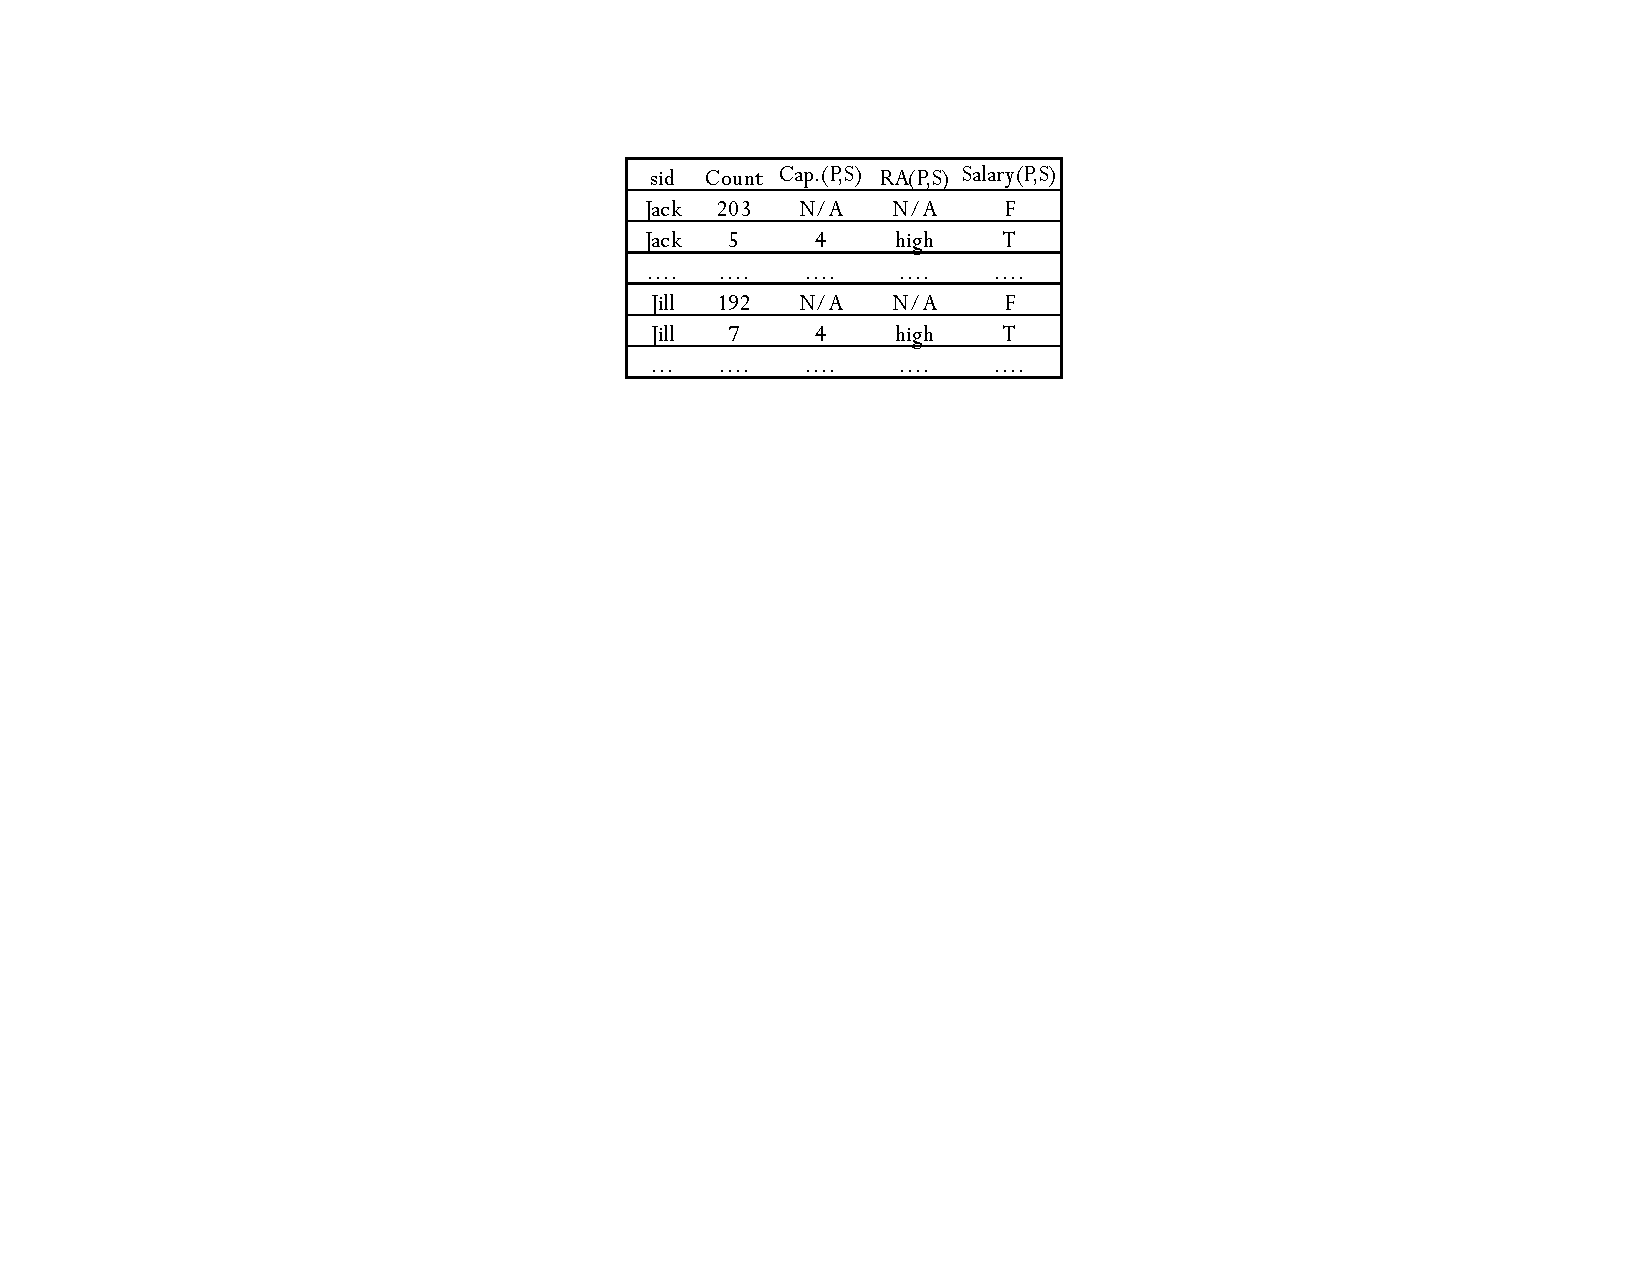
\includegraphics{targetct} 
} 
\caption{Target contingency tables for target = Jack and for target = Jill}
 \label{fig:targetc}
\end{figure}

{\em Assuming} that for each node with ID $@nodeID@$, a target contingency table $\CDB.@nodeID,target@\_\cttable$ has been built in the Count Database $\CDB$, the log-likelihood SQL is as in Section~\ref{sec:model-score}:
\begin{alltt}
SELECT @nodeID@,  SUM
(MDB.@nodeID@\_CPT.CP * CDB.@nodeID,target@\_CT.count) 
AS loglikelihood
FROM MDB.@nodeID@\_CPT NAT. JOIN CDB.@nodeID,target@\_CT
\end{alltt}
%The conditional probability database table $@nodeID,target@\_\cptable$ can be found in the Models database $\MDB$. (Notice that the conditional probabilities do not depend on the target entity, only on the model.)  
This query computes the classification score for a BN node, the total score is the sum over BN nodes. As is well-known in Bayes net theory, we need only sum scores for the target node and its children \cite{Neapolitan2004}. 
%
The new problem is finding the target contingency table. SQL allows us to solve this very easily by restricting counts to target entity in the WHERE clause. To illustrate, suppose we want to modify the contingency table query of Figure~\ref{fig:meta-query} to compute the contingency table for $\S = Jack$. We add the student id to the SELECT clause, and the join condition $S.s\_id = jack$ to the WHERE clause; see Table~\ref{table:target-query}. (Omit apostrophes for readability.) The FROM clause is the same as in Figure~\ref{fig:meta-query}. The metaquery of Figure~\ref{fig:meta-query} is easily changed to produce these SELECT and WHERE CLAUSES. 


%First we add the student id to the SELECT clause, so the new SELECT clause becomes
%
%\begin{alltt}
%COUNT(*) AS count, popularity(P), teachingability(P),
%intelligence(S), ranking(S), \em{S.sid}
%\end{alltt}
%
%and the new WHERE list becomes
%
%\begin{alltt}
%RA.p\_id = P.p\_id AND RA.s\_id = S.s\_id AND \em{S.s\_id = jack}.
%\end{alltt}

%We emphasize the new parts of the queries and omit apostrophes for readability. 
%
Next consider a setting where a model is to be scored against an entire test set. 
%This occurs for instance in the standard cross-validation computation for model scoring. 
For concreteness, suppose the problem is to predict the intelligence of a set of students
 $\it{intelligence}(jack)$, $\it{intelligence}(jill)$,
 $\it{intelligence}(student_{3}),\ldots, \it{intelligence}(student_{m})$.
 An obvious approach is to loop through the set of test instances, repeating the likelihood query above for each single instance. Instead, SQL supports {\em block access} where we process the test instances as a block. Intuitively, instead of building a contingency table for each test instance, we build a single contingency table that stacks together the individual contingency tables (Figure~\ref{fig:targetc}). Blocked access can be implemented in a beautifully simple manner in SQL: we simply add the primary key id field for the target entity to the GROUP BY list; see Table~\ref{table:target-query}. 
%To illustrate,  suppose for simplicity that the $\it{Student}$ table contains all test target entities. The query for the stacked contingency table is constructed as in Figure~\ref{fig:meta-query}, with the change that: We add the $\it{S.sid}$ field to the SELECT and to the GROUP BY lists. The FROM and WHERE clauses are as in Figure~\ref{fig:meta-query}. 
 
In contrast, programming blocked access in a general purpose programming language would require significant development effort and probably new file or data structures. If the set of test instances is large, a stacked contingency table is also unlikely to fit into main memory.
  %
To sum up, the log-likelihood computation of Section~\ref{sec:model-score} can be easily adapted to compute a log-linear classification score by adjusting the contingency table counts to the target entity. Only one or two small modifications to the log-likelihood SQL queries are required. This illustrates the modularity of MRLBase and the reusability of its components for different machine learning tasks. 


\section{Evaluation} 
We describe the system and the datasets we used.
Code was written in MySQL Script and Java, JRE 1.7.0.  and executed with 8GB of RAM and a single Intel Core 2 QUAD Processor Q6700 with a clock speed of 2.66GHz (no hyper-threading). The operating system was Linux Centos 2.6.32. 
The MySQL Server version 5.5.34 was run with 8GB of RAM and a single core processor of 2.2GHz. 
All code and datasets are available on-line (pointer omitted for blind review). 


\subsection{Datasets}
We used six benchmark real-world databases. For detailed descriptions and  the sources of the databases, please see reference~\cite{Schulte2012}. Table~\ref{table:datasetsize} summarizes basic information about the benchmark datasets.  
IMDB is the largest dataset in terms of number of total tuples (more than 1.3M tuples) and schema complexity. %attributes.
It combines the MovieLens database\footnote{www.grouplens.org, 1M version} with data from the Internet Movie Database (IMDB)\footnote{www.imdb.com, July 2013} following \cite{Peralta2007}. 

For Bayesian network structure learning, we used MRLBase to implement the previously existing learn-and-join algorithm (LAJ). The LAJ method takes as input a joint contingency table for all relational random variables in the  database, which we computed using the Count Manager. The model search strategy of the LAJ algorithm is an iterative deepening search for correlations among attributes along longer and longer chains of relationships. For more details please see \cite{Schulte2012}. 

\begin{table}[hbtp] \centering
%\scalebox{0.7in}{
\resizebox{0.5\textwidth}{!}{
\begin{tabular}[c]
{|l|c|c|r|c|}\hline
 \textbf{Dataset} & \textbf{\begin{tabular}[l] {ll} \#Relationship \\Tables/ Total \end {tabular}} & \textbf{\begin{tabular}[l] {ll} \#Self \\Relationships\end {tabular}}  & \textbf{\#Tuples} 
%& \textbf{\#Attributes}  
\\\hline
% \textbf{Dataset} & \textbf{Relationships} & \textbf{\begin{tabular}[l] {ll} Self \\Relationships \end {tabular}} &
% \textbf{\begin{tabular}[l] {ll} Same Type\\ Relationships \end {tabular}}& \textbf{\#Tuples} & \textbf{\begin{tabular}[l] {ll} \#Attribute  \\Columns \end{tabular}}  \\\hline
 %   University&2 & 0 & N & 171 & 12\\\hline
    Movielens &1 / 3 & 0  & 1,010,051 
%& 7
\\\hline
%    Movielens(0.1M) &1 & N & N &  83,402 & 7\\\hline
    Mutagenesis & 2 / 4 & 0 & 14,540 
%& 11
\\\hline
 UW-CSE &2 / 4 & \textbf{2}  & 712 %& 14
\\\hline   
  Mondial &2 / 4 & \textbf{1} &  870
%& 18
\\\hline
    %Financial &3 / 7 & 0  &  225,932& 15\\\hline
   Hepatitis &3 / 7 & 0 &12,927  
%& 19
\\\hline
   IMDB &3 / 7 & 0 &1,354,134  %& 17
\\\hline   
\end{tabular}
}
 % end scalebox
\caption{Datasets characteristics. \#Tuples = total number of tuples over all tables in the dataset. 
  \label{table:datasetsize}}
\end{table}

Table~\ref{tab:rvd} provides information about the number of relational random variables generated for each database, and the number of tuples required to store metainformation about them. More complex schemas and self-relationships lead to more random variables. 
%
%The metainformation requires little storage. The reason for using an RDBMS to store it is not because it requires large memory, but because relational algebra is an excellent language for manipulating structured objects.

% Table generated by Excel2LaTeX from sheet 'model-manager'
\begin{table}[htbp]
  \centering
    \begin{tabular}{|l|c|c|}
    \hline
   \textbf{Dataset} &\textbf{\# RRV}&  \textbf{\# Tuples in \RVD}  \\
    \hline
    Movielens & 7     & 72   \\
    \hline
    Mutagenesis & 11    & 124   \\
    \hline
    UW-CSE & 14    & 112   \\
    \hline
    Mondial & 18    & 141   \\
    \hline
    Hepatitis & 19    & 207   \\
    \hline
    IMDB  & 17    & 195   \\
    \hline
    \end{tabular}%
  %
  \caption{Random variable database statistics \label{tab:rvd}}
\end{table}%




%% Table generated by Excel2LaTeX from sheet 'Sheet1'
%\begin{table}[htbp]
%  \centering
%   \resizebox{0.5\textwidth}{!}{ \begin{tabular}{|l|r|r|r|r|r|}
%    \hline
% \textbf{  Dataset  }&  \textbf{ \begin{tabular}[l] {ll} \# Database\\Tuples  \end{tabular} }&\textbf{ \begin{tabular}[l] {ll}\# Sufficient \\ Statistics \end{tabular}}& \textbf{\begin{tabular}[l] {ll} SS \\Computing\\ Time (s) \end{tabular}} &\textbf{\begin{tabular}[l] {ll}  \#BN \\ Parameters  \end{tabular}} & \textbf{\begin{tabular}[l] {ll}Para. \\Learning\\ Time (s) \end{tabular} }\\
%    \hline
%    Movielens & 1,010,051 & 252   & 2.7   & 292   & 0.57  \\
%    \hline
%    Mutagenesis & 14,540 & 1,631 & 1.67  & 721   & 0.98  \\
%    \hline
%    UW-CSE & 712   & 2,828 & 3.84  & 241   & 1.14  \\
%    \hline
%    Mondial & 870   & 1,746,870 & 1,112.84 & 339   & 60.55  \\
%    \hline
%%    Financial & 225,932 & 3,013,011 & 1,421.87 & 2,433  & 88.974  \\
%%    \hline
%    Hepatitis & 12,927 & 12,374,892 & 3,536.76 & 569   & 429.15  \\
%    \hline
%    IMDB  & 1,354,134 & 15,538,430 & 7,467.85 & 60,059 & 505.61  \\
%    \hline
%    \end{tabular}%
%}
%  \label{tab:addlabel}%
%  \caption{Count Manager}
%\end{table}%

% Table generated by Excel2LaTeX from sheet 'Sheet1'

The number of sufficient statistics reported in Table~\ref{tab:counts}  is that for constructing the joint contingency table required for the Learn-and-Join algorithm. This number depends mainly on the number of random variables. The number of sufficient statistics can be quite large, over 15M for the largest dataset IMDB. RDBMS support is key for managing counts in such cases. Even with such large numbers, constructing contingency tables using the SQL metaqueries is feasible, taking just over 2 hours for the very large IMDB set. 
The number of Bayesian network parameters is much smaller than the number of sufficient statistics because it depends mainly on the indegree of the nodes. The Bayesian network can be seen as a compact representation of the statistical information in the joint contingency table \cite{Schulte2014}. So the difference between the number of parameters and the number of sufficient statistics measures how compactly the BN summarizes the statistical information in the data.  Table~\ref{tab:counts} shows that Bayesian networks provide very compact summaries of the data statistics. For instance for the Hepatitis dataset, the ratio is  12,374,892/569 > 20,000. The IMDB database is an outlier, showing a complex correlation pattern that leads to a dense Bayesian network structure.

\begin{table}[htbp]
  \centering
   \resizebox{0.5\textwidth}{!}{ \begin{tabular}{|l|r|r|r|r|r|}
    \hline
 \textbf{  Dataset  }&  \textbf{ \begin{tabular}[l] {ll} \# Database\\Tuples  \end{tabular} }&\textbf{ \begin{tabular}[l] {ll}\# Sufficient \\ Statistics (SS) \end{tabular}}& \textbf{\begin{tabular}[l] {ll} SS \\Computing\\ Time (s) \end{tabular}} &\textbf{\begin{tabular}[l] {ll}  \#BN \\ Parameters  \end{tabular}}%& \textbf{\begin{tabular}[l] {ll}Para. \\Learning\\ Time (s) \end{tabular} }
\\
    \hline
    Movielens & 1,010,051 & 252   & 2.7   & 292   \\%& 0.57  \\
    \hline
    Mutagenesis & 14,540 & 1,631 & 1.67  & 721   \\%& 0.98  \\
    \hline
    UW-CSE & 712   & 2,828 & 3.84  & 241   \\%& 1.14  \\
    \hline
    Mondial & 870   & 1,746,870 & 1,112.84 & 339  \\% & 60.55  \\
    \hline
%    Financial & 225,932 & 3,013,011 & 1,421.87 & 2,433  & 88.974  \\
%    \hline
    Hepatitis & 12,927 & 12,374,892 & 3,536.76 & 569   \\%& 429.15  \\
    \hline
    IMDB  & 1,354,134 & 15,538,430 & 7,467.85 & 60,059 \\%& 505.61  \\
    \hline
    \end{tabular}%
}
  \caption{Count Manager: Sufficient Statistics and Parameters \label{tab:counts}}
\end{table}%

Table~\ref{tab:model} shows that the graph structure of a Bayesian network contains a small number of edges relative to the number of parameters. 
%The reason for using an RDBMS to store the graph is again because relational algebra allows us to easily combine it with other statistical objects. 
The parameter manager provides fast maximum likelihood estimates for a given structure. This is because the variable set for a local contingency tables for BN parameter estimation comprises only a child node and its parents, so it is much smaller than the variable set in the joint contingency table.


% Table generated by Excel2LaTeX from sheet 'model-manager'
\begin{table}[htbp]
  \centering
      \resizebox{0.5\textwidth}{!}{ \begin{tabular}{|l|r|r|r|r|}
    \hline
     \textbf{ Dataset} %&  \textbf{ \begin{tabular}[l] {ll}\# Tuples In \\  RRVD \end{tabular} } 
&  \textbf{ \begin{tabular}[l] {ll} \# Tuples in \\Bayes Net  \end{tabular} }& \textbf{ \begin{tabular}[l] {ll} \# Bayes Net \\ Parameters   \end{tabular} } & \textbf{\begin{tabular}[l] {ll}Para. \\Learning\\ Time (s) \end{tabular} }\\
    \hline
    Movielens &   72    %& 12
    & 292 & 0.57  \\
    \hline
    Mutagenesis &   124   % & 57
    & 721 & 0.98  \\
    \hline
    UW-CSE &       112 %& 118
   & 241  & 1.14 \\
    \hline
    Mondial &       141 %& 126 
  & 339 & 60.55    \\
    \hline
    Hepatitis &       207%& 142 
  & 569  & 429.15   \\
    \hline
    IMDB  &      195 %& 217  
 & 60,059   & 505.61\\
    \hline
    \end{tabular}%
}  \caption{Model Manager Evaluation.}
  \label{tab:model}%
\end{table}%

Figure~\ref{fig:test-timing} compares computing predictions on a test set using an instance-by-instance loop, with a separate SQL query for each instance, vs. a single SQL query for all test instances as a block. The blocked access method is 1,000-10,000 faster. 


\begin{figure}[htbp] %  figure placement: here, top, bottom, or page
 \centering
\resizebox{0.4\textwidth}{!}{
 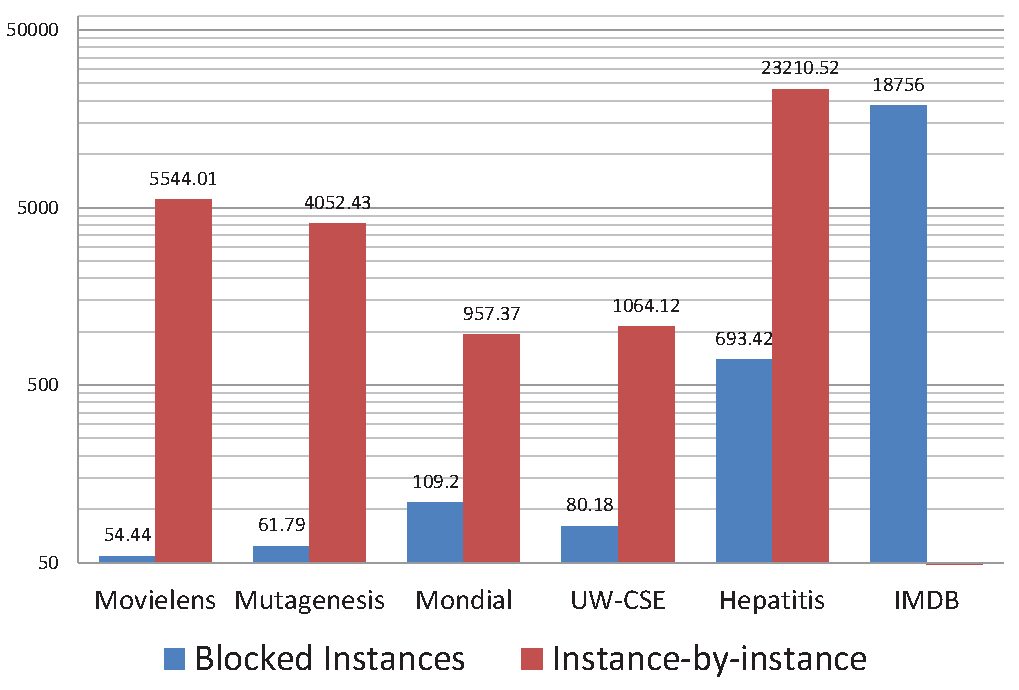
\includegraphics[width=0.5\textwidth]{test-timing.pdf} 
} 
\caption{Times (s) for Computing Predictions on Test Instances. The right red column shows the time for looping over single instances using the Single Access Query of Table~\ref{table:target-query}. The left blue column shows the time for the Blocked Access Query of Table~\ref{table:target-query}.
}
 \label{fig:test-timing}
\end{figure}

\begin{table}[htbp]
  \centering
      \resizebox{0.5\textwidth}{!}{ \begin{tabular}{|l|r|r|r|r|}
    \hline
     \textbf{ Dataset} %&  \textbf{ \begin{tabular}[l] {ll}\# Tuples In \\  RRVD \end{tabular} } 
&  \textbf{ \begin{tabular}[l] {ll} \# Tuples in \\Bayes Net  \end{tabular} }& \textbf{ \begin{tabular}[l] {ll} \# Bayes Net \\ Parameters   \end{tabular} } & \textbf{\begin{tabular}[l] {ll}Para. \\Learning\\ Time (s) \end{tabular} }\\
    \hline
    Movielens &   72    %& 12
    & 292 & 0.57  \\
    \hline
    Mutagenesis &   124   % & 57
    & 721 & 0.98  \\
    \hline
    UW-CSE &       112 %& 118
   & 241  & 1.14 \\
    \hline
    Mondial &       141 %& 126 
  & 339 & 60.55    \\
    \hline
    Hepatitis &       207%& 142 
  & 569  & 429.15   \\
    \hline
    IMDB  &      195 %& 217  
 & 60,059   & 505.61\\
    \hline
    \end{tabular}%
}  \caption{Model Manager Evaluation.}
  \label{tab:model}%
\end{table}%


Table~\ref{tab:othersrl} reports result for the complete learning of a Bayesian network, structure and parameters. It benchmarks MRLBase against functional gradient boosting, a state-of-the-art  multi-relational learning approach that construct a graphical model with parameter estimates\cite{Natarajan2012}. MLN\_Boost learns a Markov Logic Network, and RDN\_Boost a Relational Dependency Network. 
We used the Boostr implementation \cite{Khot2013}. 
To make the results easier to compare across databases and systems, we divide the total running time by the number of random variables for the database (Table~\ref{tab:rvd}). 
Table~\ref{tab:othersrl} shows that structure learning with MRLBase is fast: even the large complex database IMDB requires only around 8 minutes/node. Compared to the boosting methods, MRLBase shows excellent scalability: the competitor methods do not terminate on IMDB database, and while RDN\_Boost terminates on the MovieLens database, it is almost 5,000 times slower than MRLBase. While the Learn-and-Join algorithm is more efficient than the boosting ensemble search, much of its speed is due to quick computation of sufficient statistics. As the last column of Table~\ref{tab:othersrl} shows, on the larger datasets MRLBase spends about 80\% of computation time on gathering sufficient statistics. This suggests that a large  speedup for the boosting algorithms could be achieved if they used the MRLBase approach. 

We do not report accuracy results due to space constraints and because predictive accuracy is not the focus of this paper. On the standard conditional log-likelihood metric, as defined by Equation~\ref{eq:classify}, the BN learned by MRLBase performs better than the boosting methods on all databases. This is consistent with the results of previous studies \cite{Schulte2012}.

\begin{table}[htbp]
  \centering
      \resizebox{0.5\textwidth}{!}{
\begin{tabular}{|l|r|r|r|r|}\hline
Dataset  & RDN\_Boost  & MLN\_Boost  & MRLBase & MRLBase-CT \\\hline
MovieLens & 92.7min  & N/T & 1.12 & 0.39 \\\hline
Mutagenesis  & 118 & 49 & 1 & 0.15 \\\hline
UW-CSE & 15 & 19 & 1 & 0.27 \\\hline
Mondial  & 27 & 42 & 102 & 61.82 \\\hline
Hepatitis  & 251 & 230 & 286 & 186.15 \\\hline
IMDB & N/T & N/T & 524.25 & 439.29 \\\hline
\end{tabular}
}  \caption{Learning Time Comparison with other multi-relational learning systems. Unless otherwise noted, times are in seconds.}
  \label{tab:othersrl}%
\end{table}%

{\em Conclusion.} MRLBase leverages RDBMS capabilities for scalable management of statistical analysis objects. It efficiently constructs and stores large numbers of sufficient statistics and parameter estimates. 
%MRLBase can integrate information from different statistical objects when they are maintained as first-class citizens in the RDBMS. 
The RDBMS support for multi-relational learning translates into orders of magnitude improvements in speed and scalability.
% compared to other state-of-the-art methods.


\section{Conclusion and Future Work} 
Compared to traditional learning with a single data table, learning for multi-relational data requires new system capabilities. In this paper we described MRLBase, a system that leverages the existing capabilities of an SQL-based RDBMS to support multi-relational learning.
Representational tasks include specifying metainformation about structured random variables that are appropriate for multi-relational data, and storing the structure of a learned model. Computational tasks include storing and constructing sufficient statistics (event counts), and computing parameter estimates and model selection scores based on the sufficient statistics. 
We showed that SQL scripts can be used to implement these capabilities, with multiple advantages. These advantages include: 1) Fast program development through high-level SQL constructs for complex table and count operations. 2) Managing large and complex statistical objects that are too big to fit in main memory. 
For instance, some of our benchmark databases require storing and querying millions of sufficient statistics. 
Empirical evaluation on six benchmark databases showed significant scalability advantages from utilizing the RDBMS capabilities: Both structure and parameter learning scaled well to millions of data records, beyond what previous multi-relational learning systems can achieve. 
%For the important task of computing prediction scores for test instances, block access provided by the RDBMS runs orders of magnitude faster than a loop through test instances. 

{\em Future Work.} On the RDBMS side, our implementation has used simple SQL plus indexes. Further optimizations are likely possible, especially for view materialization and the key scalability bottleneck of computing multi-relational sufficient statistics. An important direction is to integrate MRLBase with probabilistic inference systems that also utilize RDBMS capabilities, such as BayesStore and Tuffy. Further potential application areas for MRLBase include managing massive numbers of aggregate features for classification \cite{Popescul2007}, and collective matrix factorization \cite{Singh2008}. 
%Another research direction is to exploit the capabilities of other advanced data management system for multi-relational learning, in addition to multi-relational databases. These include OLAP systems for hierarchical structures and Hadoop systems for distributed computations. 

In sum, we believe that the succesful use of SQL presented in this paper shows that relational algebra can play the same role for multi-relational learning as linear algebra for single-table learning: a unified language for both representing statistical objects and for computing with them.
% The following two commands are all you need in the
% initial runs of your .tex file to
% produce the bibliography for the citations in your paper.
\bibliographystyle{abbrv}
\bibliography{master,master1,master2,master3,master4} 



%ACKNOWLEDGMENTS are optional
%\section{Acknowledgments}
%
%This research was supported by a Discovery grant to Oliver Schulte by the Natural Sciences and Engineering Research Council of Canada. 
%Zhensong Qian was supported by a grant from the China Scholarship Council.
%We thank the organizers for providing a discussion venue, and the anonymous reviewers for constructive criticism.




 % vldb_sample.bib is the name of the Bibliography in this case
% You must have a proper ".bib" file
%  and remember to run:
% latex bibtex latex latex
% to resolve all references

%\subsection{References}

%%APPENDIX is optional.
%% ****************** APPENDIX **************************************
%% Example of an appendix; typically would start on a new page
%\newpage
%\pagebreak
%



\end{document}


